\documentclass[german,version-2020-11]{uzl-thesis}


% Copy this file as a template for your thesis. You will have to take
% action at all places marked by
%
% !!!!!!!!!!!!!!!!!!!!!!!!!!!!!!!!!!
% !!! Your action is needed here !!!
% !!!!!!!!!!!!!!!!!!!!!!!!!!!!!!!!!!
%
% The first place your action is needed is the first line of this
% document:
%
%
% Language of the thesis:
%
% You must use either 'german' or 'english' above, depending on the
% language used in the main text. This will automatically setup a lot
% of things in the background.
%
%
% Version of the class:
%
% You must specify which version of the thesis class is to be
% used. This is important in case the class style changes in later
% years, but we still want an older thesis to look the same, even when
% things are changed in the class.
%
% Do not change or remove the version-xxxx key.
%
%
% Text encoding:
%
% Your thesis *must* be encoded in utf8 (unicode), which is the
% default in most editors these days. Do *not* change this to latin8.



%%%
%
% Main setup:
%
%%%
%
% You must use the \UzLThesisSetup command to specify numerous things
% about your thesis. This includes the entries on the title page, the 
% abstracts, and the bibliography style. You do so by specifying
% so-called "values" for so-called "keys". For instance, 
% for the key "Autor" you must provide your name as the value. You do
% so by writing 'Autor = {Max Mustermann}', that is, the value is put
% into curly braces. You can use the \UzLThesisSetup command
% repeatedly and the order in which you provide the keys is not
% important. 
%
% Everything shown on the title page must be in German -- even
% if the thesis is written in English! Just insert German text for
% German keys and English text for English keys (like 'Abstract' needs
% English text, while 'Zusammenfassung' needs German text).

\UzLThesisSetup{
  %
  % !!!!!!!!!!!!!!!!!!!!!!!!!!!!!!!!!!
  % !!! Your action is needed here !!!
  % !!!!!!!!!!!!!!!!!!!!!!!!!!!!!!!!!!
  %
  % First, specify the institut or clinic at which the thesis was
  % written. You get the logo file from them (make sure it has the
  % correct size, namely the same as the example). If they do not have
  % a logo, the university's default logo is used.
  %
  % The 'verfasst' gets two arguments. Change the first to {an der}
  % for clinics, as in 'Verfasst = {an der}{Medizinischen Klinik I}'
  %
  Logo-Dateiname        = {uzl-thesis-logo-itcs.pdf},
  Verfasst              = {am}{Institut für Informationssysteme},
  %
  % The titles:
  %
  Titel auf Deutsch     = {
    Topic-Modellierung für die Zuordnung von Kundenanfragen zu Sachbearbeitern
  }, 
  Titel auf Englisch    = {
    Topic modeling for the assignment of customer inquiries to clerks
  },
  %
  % Author and supervisor:
  % 
  % Note that the 'Betreuer' or 'Betreuerin' is the supervisor, that
  % is, the professor who officially supervises the thesis. If there
  % is also an assistent of the professor who helped (typically a
  % lot), use 'Mit Unterstützung von' to thank that person. If the
  % thesis was mainly written 'externally' at some company or another
  % institute, point this out using 'Weitere Unterstützung'. 
  % 
  % For your own name, do *not* add things like "BSc" or "BSc
  % cand.". For the supervisor, you should normally include
  % "Prof. Dr." or "PD Dr." (ask your supervisor, what is
  % appropriate), but nothing more (so no
  % "Univ.-Prof. Dr. Dr. h.c. mult." unless your supervisor insists).  
  %
  Autor                 = {Leonard Brenk},
  Betreuerin            = {Prof. Dr. Ralf Möller},
  % 
  % Optional: Supporting persons and institutions. The text should be
  % in German, even for an English thesis.
  %
  Mit Unterstützung von = {Dr. Jinghua Groppe, Felix Kuhr, Magnus Bender},
  % 
  %   Weitere Unterstützung = {
  %     Die Arbeit ist im Rahmen einer Tätigkeit bei der Firma Muster GmbH
  %     entstanden.
  %   },
  %
  %
  % Your Degree Programm (Studiengang)
  %
  % Specify 'Bachelorarbeit' or 'Masterarbeit' and the degree
  % programme. Make sure the name of programme is correct and not
  % some abbreviation or some incorrect variant. For instance:
  % 'Medizinische Ingenierwissenschaft', but not 'MIW';
  % 'Medizinische Informatik', but not 'Medizin-Informatik';
  % 'Informatik', but not 'Informatik (SSE)'.
  %
  % Use German names for German programmes and English names for
  % English ones, so 'Infection Biology', not 'Infektionsbiologie'. 
  % For programmes that have a German bachelor and an English master,
  % use the German name for a bachelor thesis and the English name for
  % the master thesis.
  %
  Bachelorarbeit,
  Studiengang           = {Informatik},
  %
  % Date on which the thesis is turned in German, formatted the
  % traditional German way:
  %
  Datum                 = {1. Oktober 2021},
  %
  % The English abstract. You must always provide abstracts in German
  % and in English. 
  %
  Abstract              = {
   Every day, huge amounts of data are generated that need to be organized, stored and understood. Topic modeling methods are ideal for this purpose. In this process, words that frequently occur together are grouped into a topic. Probably the best known method is Latent Dirichlet Allocation (LDA), which is applied in this work to data from the Zentralverband Ostholstein (ZVO). The ZVO is a company that is active in the field of supply and disposal in northern Germany. Every year, it receives many e-mail inquiries from customers, which are currently divided manually into 18 departments. In the future, this should be done automatically by an algorithm. For this application, the quality of the data is analyzed in this thesis. For this purpose 18 topics are generated by an LDA model and their overlaps with the manually created departments are examined. The result is that the departments are too similar and have many identical words and phrases. In addition, some of the departments contain too little data to identify distinct patterns in them. Thus, regarding the current data of ZVO, topic modeling is not a suitable variant for classification.
  },
  Zusammenfassung       = {
      Täglich werden riesige Mengen an Daten erzeugt, die organisiert, gespeichert und verstanden werden müssen. Dafür bieten sich Methoden der Topic-Modellierung an. Dabei werden Wörter, die häufig zusammen vorkommen zu einem Topic, also einem Thema, gruppiert. Die wohl bekannteste Methode ist die Latent Dirichlet Allocation (LDA), die in dieser Arbeit auf Daten des Zentralverbands Ostholstein (ZVO) angewendet wird. Der ZVO ist ein Unternehmen, dass sich in Norddeutschland in dem Bereich der Ver- und Entsorgung betätigt. Er bekommt jährlich viele E-Mail-Anfragen von Kunden, die momentan händisch in 18 Abteilungen eingeteilt werden. Das soll in Zukunft automatisiert durch einen Algorithmus geschehen. Für diese Anwendung wird in dieser Arbeit die Qualität der Daten analysiert. Dafür werden 18 Topics von einem LDA Modell generiert und deren Überschneidungen mit den händisch erstellen Abteilungen untersucht. Die Erkenntnis ist, dass die Abteilungen zu ähnlich sind und über viele identische Wörter und Phrasen verfügen. Außerdem wird in der Arbeit festgestellt, dass ein Teil der Abteilungen zu wenig Daten enthält, um eindeutige Muster in diesen zu erkennen. Für die aktuellen Daten der ZVO stellt Topic-Modellierung somit keine geeignete Variante zur Klassifizierung dar.
  },
  %
  % Optional: 'Danksagungen' (German) or 'Acknowledgements'
  % (English). Both keys are optional and both have the same effect of
  % adding an acknowledgements text after the abstracts and before the
  % table of contents.
  \begin{comment}
  Acknowledgements      = {
    This is the place where you can thank people and institutions, do
    not try to do this on the title page. The only exception is in
    case you wrote your thesis while working or staying at a company or abroad. Then you
    should use the \Latex{Weitere Unterstützung} key to provide a text
    (in German) that acknowledges the company or foreign
    institute. For instance, you could use texts like »Die Arbeit
      ist im Rahmen einer Tätigkeit bei der Firma Muster GmbH
      entstanden« or »Die Arbeit ist im Rahmen eines
      Forschungsaufenthalts beim Institut für Dieses und Jenes an der
      Universität Entenhausen entstanden«. Do not name and thank
      individual persons from the company or foreign institute on the
      title page, do that here. 
  },\end{comment}
  % Bibliography style: Choose between
  % 
  % 'Alphabetische Bibliographie'
  % for all degree programmes in the natural sciences 
  % 
  % 'Numerische Bibliographie'
  % alternative for all other degree programmes
  % 
  % Either will load biblatex and setup the citation methods and the
  % bibliography styles correctly. You should not mess with them.
  % 
  Alphabetische Bibliographie,
  % Alternatively:
  % Numerische Bibliographie
}




%%%%%%%%%%%%%%%%%%%%
%
% Styling the thesis
%
%%%%%%%%%%%%%%%%%%%%
%
% Creating a visually pleasing layout and choosing fonts is not
% easy. Furthermore, different people have different preferences. Of
% course, for the University of Lübeck, the dean of studies could just
% force everyone to use one specific layout and font, but that seems a
% bit drastic and, also, it seems nice that thesis by different people
% have an individual style even though they all stick to the same
% overall structure.
%
% For these reasons, I (Till Tantau) have spend quite some time on
% designing a flexible layout and styling mechanism for theses.
%
% Basically, the overall structure of the thesis is fixed by the
% thesis class and so are many structural elements. For instance, you
% cannot change the order in which the abstract and table of contents
% are shown, you cannot move the bibliography elsewhere, indeed, the
% bibliography style is also fixed. Likewise, the text on the title
% page is fixed.
%
% Although many things are fixed, you *can* change several other
% things. For instance, you can change the font used for the main
% text, you can change which font is used for titles and headings or
% you can change whether titles and headlines are centered or flushed
% left.
%
% There are many LaTeX packages for changing such things. You are
% kindly asked *not to use them*. Rather, use (only) the options
% offered by the thesis class. All possible choices and combinations
% there have been tested by me and produce nice results; what happens
% with other packages no one knows and might no longer conform to what
% is expected by the university. As you will see, you still have a
% lot of options.
%
%
% Technical note: All styling is done via the command
%
% \UzLStyle{...}
%
% where ... is a key-value list just as for \UzLThesisSetup. The
% difference is just that everything having to do with styling as
% controlled by \UzLStyle, while the more “formal” setup keys are
% controlled by \UzLThesisSetup.
%
%%%
%
% Designs
%
%
% A \emph{design} is a whole set of font and layout options bundled
% together. They have been chosen in such a way that a visually
% pleasing “overall appearance” results.
%
%
% \UzLStyle{computer modern oldschool design}
%
% The look of this design mimics the “classical” way a paper or report
% created with \LaTeX\ looks like: The Computer Modern font is used,
% bold face fonts are used for headlines, only black and white are
% used as colors. This design reminds me of older scientific
% documents, especially from the computer science community where
% \LaTeX\ was used very early.
%
%
% \UzLStyle{computer modern basic design}
%
% A slightly less “oldschool” version of the previous design. It is
% still a classic design in the sense that it uses the Computer Modern
% font and that it still has this “good old \LaTeX” look, but some
% more modern aspects (like colors!) have been added.
%
% Note that this design uses Myriad for the title page (one of the
% “modern aspect”), which means that his font must be installed.
%
%
%\UzLStyle{computer modern scholary design}
%
% In my opinion, this is the ultimate “scholary design”: The thesis
% will look like it has been typeset by hand some 150 years ago and
% then printed by a university press. There is really nothing “modern”
% about it and the word in the name of the design is just part of the
% name of the “Computer Modern” font.
%
%
% \UzLStyle{pagella basic design}
%
% A, well, basic design that uses the Pagella font rather than the
% Computer Modern font. Especially the bold face version of this font
% looks nicer than the Computer Modern counterpart. Also, Pagella,
% while still having a “bookish” look, still feels a bit fresher than
% Computer Modern. 
%
%
% \UzLStyle{pagella centered design}
%
% A variant of the basic Pagella design that centers all
% headlines. A nice alternative to the basic version.
%
%
\UzLStyle{pagella contrast design}
%
% This design tries to create some visual friction by contrasting the
% sans serif headline font (in bold!) with the main text. I find it a
% visually very interesting combination.
%
%
% \UzLStyle{alegrya basic design}
%
% The third variant of the basic design, this time using the Alegrya
% font. 
%
%
% \UzLStyle{alegrya scholary design}
%
% The Alegrya version of the previous “scholary” design. Unlike the
% Computer Modern version, this design does not look old, but more
% fresh -- while still creating the impression that the text must be
% about a very scientific subject. 
%
%
% \UzLStyle{alegrya stylish design}
%
% The design is quite similar to the scholary version for the Alegrya
% font, but with even more modern additions. “Stylish” is the word
% that comes to my mind.
%
%
%\UzLStyle{alegrya modern design}
%
% A design that uses the sans serif version of the Alegrya font for
% the headlines. This is a nice modern overall design.
%
%%%




%%%%%%%%
%
% Now, include the package you need here using \usepackage. 
%
% However, many standard packages are already loaded by the class:
%
% amsmath, amssymb, amsthm, babel, biblatex, csquotes, etoolbox,
% filecontents, fontspec, geometry, hyperref, tikz (with libraries
% arrows.meta, positioning and shapes), varioref, url 
%
% Indeed, in many cases you will not need any extra packages.
%
%%%%%%%


\usepackage{graphicx}
\usepackage{listings}
\usepackage{xcolor}
\usepackage{comment}
\usepackage{tikz}
\usepackage{amsmath}
\usetikzlibrary{arrows, automata, positioning}
\usepackage{pgfplots}
\usepackage{algorithm2e}
\usetikzlibrary{shapes,arrows}
\usetikzlibrary{shapes.geometric, arrows}
\usepackage{algorithm}
\usepackage{algorithmic}
\usepackage{caption}
\usepackage{float}


\begin{document}

%
% The title page and table of contents will be inserted automatically
% here. 
%


\chapter{Einleitung}%%%%%%%%%%%%%%%%%%%%%%%%%%%%%%%%%%%%%%%%%%%%%%%%%%%%%EINLEITUNG
% In a German thesis write: \chapter{Einleitung}


% !!!!!!!!!!!!!!!!!!!!!!!!!!!!!!!!!!
% !!! Your action is needed here !!!
% !!!!!!!!!!!!!!!!!!!!!!!!!!!!!!!!!!
%
% Replace with your own introduction:

% DELETE the following line for your own thesis - it causes trouble!
\lstMakeShortInline[style=code,style=inline,language={[LaTeX]tex},moretexcs={chapter}]|


Die digitalisierte Welt generiert täglich riesige Mengen an neuen Informationen. Von E-Books, Blogs über Nachrichten-Websites und Magazinen bis hin zu mobilen Anwendungen auf dem Smartphone, immer mehr Menschen verlassen sich auf und richten ihr Leben nach dem Internet aus. Das Zeitalter des Big-Data ermöglicht es Nutzern unbegrenzt viele Daten zu generieren und zu sammeln. Die Kapazitäten, die ein Mensch aufbringen kann, um solche Massen an Daten zu organisieren und zu verstehen, sind schon lange übertroffen. Vor allem durch die steigende digitale Kommunikation und stetig sinkenden Speicherplatzkosten, erhöht sich die Menge an zu speichernden Einsen und Nullen. Laut Statista \cite{statista}  wurden 2018 33 Zettabyte an Daten generiert mit einer prognostizierten Steigerung bis 2025 um 530\% auf 175 Zettabyte. Dieser dramatische Anstieg zeigt die Dringlichkeit für effiziente Algorithmen und Methoden der Datenverarbeitung. Neben der reinen Handhabung solcher Daten steigt aber auch das Bewusstsein, aus diesen Daten Verständnis und Potentiale zu schaffen. Besonders Suchverfahren gewinnen an Bedeutung, wenn in großen, unübersichtlichen Datenmengen bestimmte Informationen gefragt sind. Für die Mehrheit bieten Firmen, wie Google, diese Anwendung an. Zwar kann durch die Keyword-basierten Suche das passende Dokument gefunden werden, jedoch schlägt die Suchmaschine fehl, wenn nach einer Menge von Dokumente mit einem übergreifenden Thema gefragt ist. Um mehrere Dokumente auf geteilte Themen zu untersuchen, wird die sogenannte Topic-Modellierung verwendet. Topic-Modellierung (dt. Themenmodellierung) beschreibt eine Gruppe von Verfahren, die es ermöglichen, große elektronische Datensammlungen automatisiert zu durchsuchen, zu organisieren und zu verstehen. Es können Muster innerhalb der Daten entdeckt und Topics extrahiert werden. Ein Topic stellt dabei eine Menge an Wörtern dar, häufig gemeinsam in einem Kontext vorkommen. Einem Topic über Hunde würden beispielsweise die Wörter Bellen, Fell und Halsband zu einer hohen Wahrscheinlichkeit angehören, da sie oft gemeinsam in dem übergeordneten Thema über Hunde gebraucht werden. Die Modellierung solcher Topics wird als Topic-Modellierung bezeichnet, da in einer Datenmenge nach mehreren solcher Topics gesucht wird. Diese können zu unterschiedlichen Anteilen in dem Dokument vertreten sein. Ein Dokument ist dabei ein Teil eines Korpus, also einer Menge mehrerer Dokumente. Dabei stellen Topic-Modelle statistische Modelle dar, die Verwendung in der Inferenz abstrakter Topics in unsortierten Datenmengen finden. Topic Modelling gehört zu dem Bereich des Natural Language Processing, also der Verarbeitung natürlicher Sprache. Es verbindet Computerlinguistik, Informatik und Künstliche Intelligenz, um die Potentiale der Sprachverarbeitung mit der heutigen Technik auszuschöpfen. In einer Welt von exponentiell wachsenden Datenmengen finden Methoden der Topic-Modellierung stetig eine breitere Anwendung. Bereits heute wird Topic-Modellierung in vielen Bereichen der Wirtschaft, Wissenschaft und Informationstechnologie verwendet. So findet die Topic-Modellierung unter anderem Anwendung bei Zusammenfassungen, Spam Filtern, Internet of Things (IOT), Healthcare, Blockchain, Chatbots, FAQs oder HR. Dies zeigt wie umfangreich das Anwendungsspektrum der Topic-Modellierung ist. Um semantische Folgerungen aus Datenmengen zu generieren, gibt es verschiedene Ansätze – in dieser Arbeit wird es um die generative Methode Latent Dirichlet Allocation(LDA) gehen. Dabei werden ähnliche Wörter, die in ähnlichen Kontexten vorkommen in Topics gruppiert. Die Grundlagen des LDA liegen bei der Verallgemeinerung des bereits $1999$ veröffentlichten Probabilistic Latent semantic Analysis (PLSA). Im Gegensatz zu anderen Machine Learning Methoden im Bereich der Datenverarbeitung, hat Topic-Modellierung die Besonderheit, dass ein Dokument nicht nur zu einem Topic zugeordnet werden kann, wie z.B. bei Clusteralgorithmen. Bei der Topic-Modellierung wird jedes Dokument durch eine Verteilung an Topics beschreiben, das bedeutet in jedem Dokument sind immer alle Topics zu finden - nur zu einem bestimmten Anteil. Genauso sind in einem Topic immer alle Worte zu einer bestimmten Wahrscheinlichkeit vorhanden. Bei einem Artikel, der zu $90\%$ über Sport und $10\%$ über Politik handelt, werden somit neun mal mehr Wörter bezüglich Sport zu finden sein, als über Politik. Topic-Modellierung wird den unüberwachten Lernmethoden des Data Minings zugeordnet, also der Extraktion von Muster und Trends in Datenmengen durch die Anwendung statistischer Algorithmen. Das bedeutet, dass die Topics ohne die Einwirkung von manuell erzeugten Labels gefunden werden. Im Lernprozess werden dann Verteilungen basierend auf den bislang vorgenommenen Zuordnungen iterativ angepasst und verbessert - jedoch alles ohne menschliches Zutun. 

\section{Ziel}
Diese Arbeit wird die Theorie der Topic-Modellierung anhand des Beispiels des Zweckverband Ostholstein (ZVO) in der Praxis implementieren und die bezüglichen Parameter im Sinne des ZVO bewerten. Der ZVO ist ein Unternehmen, das in Norddeutschland in der Energie-, Entwässerungs-, Internet- und Entsorgungsbranche tätig ist.  Es erhält jährlich ein große Menge an Kundenanfrage, die von Mitarbeitern gelesen und klassifiziert wird. Die klassifizierte Kundenanfrage wird dann an die zuständige Abteilung weitergeleitet. Dieser Vorgang ist sowohl zeitintensiv, als auch fehleranfällig und führt zu einer Ineffizienz in der Wertschöpfungskette. Der Prozess soll zukünftig automatisch durch einen Klassifikationsmechanismus funktionieren. \\
Diese Arbeit verfolgt zwei Ziele: 
\begin{enumerate}
\item Vorhersage der Qualität der Klassifikation durch Untersuchung der Datenqualität
\item Analyse der vordefinierten Abteilungen durch Topiczuordnung
\end{enumerate}

Diese Arbeit beschäftigt sich mit der Vorhersage der Qualität des Klassifikators, indem die Qualität der manuell erstellten Kategorien und Kundenanfrage-Gruppen untersucht und mit den Ergebnissen verschiedenen Topic Modellierungen verglichen wird. Das Ergebnis eines Topic Models hängt stark von der Qualität der Daten ab, die sie als Input bekommt. Diese Daten durchlaufen eine Reinigungsphase, bevor sie klassifiziert werden, um sie in eine gut zu verarbeitende Form zu bringen. Der Prozess der Reinigung kann Einfluss auf das Ergebnis haben. Ziel dieser Arbeit ist es, Erkenntnisse über die Qualität des Klassifikators zu treffen, in Abhängigkeit zu den verwendeten Daten. Somit wird durch die Nutzung von LDA-Modellen die Qualität der Daten untersucht und Prognosen über einer höheren Qualität der Klassfikiation anhand der Daten getroffen. 

\section{Sturktur dieser Arbeit}
Der Bereich Data Science und Datenverarbeitung durchläuft aktuell eine starke Welle an Innovation und Veränderung. Deshalb wird in dieser Arbeit zuerst eine Einleitung die Motivation und das Prinzip der Topic-Modellierung beschreiben. Gefolgt wird die allgemeine Einleitung von der Motivation und Aufgabenstellung in Bezug auf das Anwendungsbeispiel des Zweckverbands Ostholstein (ZVO). Die Anwendung der Algorithmen wird im Laufe der Arbeit mit theoretischen Grundlagen erklärt, die eine klare Notation fordern: diese ist im Teil der Notationen gelistet. Das Prinzip der Topic-Modellierung kann mit unterschiedlichen Ansätzen implementiert werden. Beispiele sind: LDA, NNF und LSA. Da sich diese in ihrem Ansatz und in ihrer Umsetzung unterscheiden, werden im nächsten Abschnitt die bekanntesten dieser Modelle verglichen, indem ihre Vorgehens- und Funktionsweise untersucht werden. Die Methode, die in dieser Arbeit genauer beleuchtet wird, ist Latent Dirichlet Allocation. Der dritte Abschnitt wird von der Herkunft, dem Format und der Verarbeitung der Daten der ZVO handeln. Dabei wird der Anwendungsfall und die ZVO genauer erklärt und ein Einblick in die Daten, deren Reinigung und Verarbeitung gegeben. Darauf folgt das Konzept der Lösungsstrategie, um die Aussagekraft und Qualität der Daten für Topic-Modellierung erfolgreich zu untersuchen. Dafür wird der Ablauf des Algorithmus anschaulich dargestellt und die Prozesskette der Analyse im Detail aufgeschlüsselt. Im vierten Abschnitt findet die Implementierung des im dritten Abschnitt erklärten Konzepts statt. Für diese wird eine Methode der Topic-Modellierung ausgewählt und in einer vorher definierten und begründeten Programmierumgebung realisiert. Die Umsetzung wird anhand des gelisteten Algorithmus zeilenweise erklärt. Der Output ist in die Arbeit integriert, um dessen zentrale Rolle in der Datenanalyse zu unterstreichen und die Ergebnisse verständlich begründen zu können. Die detaillierte Analyse folgt im nächsten Abschnitt, der sich damit befasst, die Ergebnisse der Implementierung im Anwendungsfall der ZVO zu interpretieren. Dabei wird begründet, wie gut sich die Daten für eine Topic-Modellierung eignen und was die Ergebnisse über die Qualität der Daten aussagen. Die Arbeit wird abgeschlossen mit der Zusammenfassung und einem Ausblick für die ZVO in Bezug auf Topic-Modellierung. Die gewonnenen Ergebnisse der Datenqualität sollen der ZVO nach der Ergebnisgewinnung zu einer höheren Effizienz in der Datenverarbeitung verhelfen und Aufschluss über Handlungsbedarf und Optimierungspotential in den Datensätzen geben.


\chapter{Grundlagen}%%%%%%%%%%%%%%%%%%%%%%%%%%%%%%%%%%%%%%%%%%%%%%%%%%%%%%%%%%%%GRUNDLADEN

In diesem Kapitel werden die grundlegenden Eigenschaften von Topic-Modellierung erklärt. Dabei wird auf die verschiedenen Methoden Bezug genommen und Parameter erklärt, die beeinflussen können, wie eine Methode Topics erkennt und klassifiziert. Topic-Modellierung wird schon seit vielen Jahren verwendet und hat viele Veränderungen durchlaufen. Diese Arbeit wird in diesem Kapitel auf die wichtigsten Entwicklungsmeilensteine eingehen.

\section{Notation}
Für das Verständnis von Topic-Modellierung ist es wichtig die Begriffe zu kennen und zu verstehen. Dabei sind Wörter bekanntermaßen Mengen aus beliebigen Buchstaben. Mehrere Wörter bilden zusammen ein Dokument. Mehrere Dokumente werden als Korpus bezeichnet. Dokumente können Topics, also Themenbereiche, zu unterschiedlichen Anteilen abdecken. Topic-Modellierung versucht diese Topics aus Dokumenten zu extrahieren.

\begin{itemize}
	\item Ein Wort wird mit $w \in N$ mit $N$ als Menge aller Worte bezeichnet
	\item Eine Menge Wörter ergeben ein Dokument $d \in D$ mit $D$ als Menge von Dokumenten
	\item Eine Menge an Dokumenten ergibt einen Korpus $D$
	\item Eine Menge an Wörtern ergibt eine Topic $z \in K$ mit $K$ als Menge aller Topics
	\item Ein Topic-Modell wird mit $M$ beschrieben
\end{itemize}


\section{Techniken der Topic- Modellierung}

Das Feld des Information Retrieval bietet vielseitige Verfahren, um Topic-Modellierung zu betreiben. Bei vielen geht es um eine Dimensionsreduktion des Datensatzes, die Aufschluss und Erkenntnis über die Datenmenge geben soll, indem sie in eine weniger komplexe Darstellungsform umgewandelt werden. In dieser Arbeit wird die Latent Dirichlet Allocation(LDA) verwendet, das als Bindeglied zwischen statistischen und probabilistischen Maßen agiert. LDA wurde durch die Optimierung und Vermischung verschiedener vorangegangener Verfahren entwickelt. Die wichtigsten Verfahren in der Entwicklung von LDA sind im Folgenden aufgelistet und erklärt: 

\subsection{Term Frequency - Inverse Document Frequency(Tf-idf)}
Das Verfahren der (Tf-idf) beschreibt ein statistisches Maß, um die Wichtigkeit von Wörtern in einer Gruppe von Dokumenten zu beurteilen. Die Term-Frequency(Tf) erstellt eine Matrix, die die Anzahl der Wörter auf die Dokumente abbildet, in denen sie enthalten sind. Um zu vermeiden, dass Wörter, die wenig Aussagekraft für den Korpus haben, wie das Wort \glqq und\grqq, bestimmt die Inverse Document Frequency(idf) wie spezifisch ein Wort für einen gesamten Korpus ist. Das einzelne Dokument ist dafür demnach nicht mehr wichtig. Die Idee dabei ist, dass Wörter, die sehr selten vorkommen ein Dokument unter Umständen stärker beeinflussen können, als ein Wort, das so häufig vorkommt, dass es schon keine Aussagekraft oder semantische Relevanz mehr hat. Das Verfahren verwendet keine probabilistischen Elemente sondern ist eine rein statistische Möglichkeit herauszufinden, wie wichtig ein Wort eines Dokuments für das Gesamtthema des Dokuments ist. 

\subsection{Latent Semantic Analysis}
Viele Verfahren der Topic-Modellierung gehen auf das sogenannte Latent Semantic Analysis (LSA) zurück, das zuerst 1990 erwähnt wurde. LSA baut auf dem Prinzip der Tf-idf auf, indem es die Tf-Matrix nutzt und adaptiert. Bei dem Verfahren geht es um das Finden von sogenannten Hauptkomponenten in Dokumenten. Grob können Hauptkomponenten als allgemeine Überthemen verstanden werden. So wäre Politik die Hauptkomponente, die von Wörtern wie Politiker, Bundestag und Regierung beschrieben wird. Mathematisch gesehen verbindet man mit der Hauptkomponente die Hauptkomponentenanalyse, die als statistische Methode versucht, viele Variablen mithilfe von Eigenvektoren und Kovarianzen in einer vereinfachten Form mit einem möglichst geringen Informationsverlust darszustellen. Dabei ist das Ziel die Tf-Matrix möglichst verkleinert darzustellen, die die Anzahl der Vorkommen für jedes Wort pro Dokument abbildet. Sie wird in Matrizen aus Eigenvektoren und Eigenwerten aufgespalten, wodurch es möglich ist, die wichtigen Hauptkomponenten aus der meist sehr großen Tf-Matrix zu extrahieren. Diese Matrix wird als Produkt von drei Matrizen dargestellt, von denen die mittlere eine Diagonalmatrix darstellt. Die Werte auf der Diagonalen lassen daraus die Topics der Textmenge ablesen. LSA stellt sich als ein attraktives Verfahren heraus, da es Synonyme besser erkennen kann als LDA und wird heutzutage unter anderem intensiv in dem Bereich des Digital Marketings genutzt. 

\subsection{Probabilistic Latent Semantic Analysis}
Probabilistic Latent Semantic Analysis (PLSA) verfolgt den Ansatz, ein Wahrscheinlichkeitsmodell zu finden, das ein Dokument erzeugt, dass zu der Tf-Matrix passt. PLSA hat als erste Methode dem Konzept der Topic-Modellierung Wahrscheinlichkeiten hinzugefügt. Dabei sind das Dokument und Wort bekannt, das assoziierte Topic jedoch nicht. Der grundlegende Gedanke ist, dass ein Dokument generiert werden kann, indem zuerst das Dokument mit einer bestimmten Wahrscheinlichkeit gewählt wird, dann ein Topic und aus diesem Topic dann ein Wort - alles mit Wahrscheinlichkeiten beschrieben. Es lässt sich der Fall, dass Dokument $d$ über Topic $z$ handelt, mit einer Wahrscheinlichkeit von $P(z \mid d)$ beschreiben. Dazu berechnet $P(w \mid z)$, wie wahrscheinlich es ist, dass das Wort $w$ aus einem gegebenen Dokument $d$ zu Topic $z$ gehört. Somit führt PLSA die Gesamtwahrscheinlich ein, dass ein Wort in einem gegebenen Dokument zu finden ist: $P(D,W) = P(D) \sum_{Z}{P(Z\mid D)P(W\mid Z)}$. Die Gleichung verbindet die Wahrscheinlichkeit ein bestimmtes Dokument zu erhalten mit der eines Wortes in diesem bedingt durch die Topic-Verteilung in diesem Dokument. 

\subsection{Latent Dirichlet Allocation}
Basierend auf LSA und PLSA ergibt sich eine der meist verbreiteten Verfahren, das Latent Dirichlet Allocation (LDA). Dieses Verfahren ist sehr ähnlich zu PLSA, das durch zwei Dirichlet-Verteilungen ergänzt wurde. LDA liegt, genau wie PLSA, ein generierender Prozess zugrunde, der jedes Dokument basierend auf mehreren Wahrscheinlichkeitsverteilungen generieren kann. Dabei wird zuerst das Dokument $d$ mit $P(d)$ gewählt, für dieses dann eine Topic $z$ mit $P(z \mid d)$ und anschließend die Wörter w mit $P(w \mid z)$. Grundsätzlich werden Dokumente bei LDA als die Dokument-Topic-Verteilung dargestellt, die die Ausprägungen verschiedener Topics in einem Dokument beschreibt. Für die Topics gibt es die Topic-Word-Verteilung, die die Wahrscheinlichkeit beschreibt, dass ein bestimmtes Wort in einer gewissen Regularität in einem Topic vorkommt. Dabei geht man davon aus, dass ein Dokument eine Verteilung von Topics ist, während ein Topic als eine Verteilung über Wörter betrachtet wird. Der Unterschied zu PLSA liegt in zwei hinzugfügten Dirichlet Verteilungen, die die Zuordnung von Dokumenten zu Topics maßgeblich beeinflussen.
Die Wahrscheinlichkeit, dass ein bestimmtes Dokument generiert wird, ist das Produkt der Wahrscheinlichkeiten der Dokument-Topic-Verteilung und Topic-Word-Verteilung mit den Wahrscheinlichkeiten der zwei hinzugefügten multinomialen Dirichlet-Verteilungen. So werden erst die Topics zufällig ausgewählt, wie in der Dirichlet-Verteilung definiert, und aus diesen dann, mithilfe der zweiten Dirichlet-Verteilung, Wörter aus diesen Topics hergeleitet, wodurch das Enddokument entsteht. Die Herangehensweise ist in der Realität meistens umgekehrt, da selten Dokumente auf basis bekannter Topics generiert werden müssen, sondern eher Topics von bekannten Dokumenten gefunden werden sollen. 

%\subsection{Non-Negative Matrix Factorization}
%Ein weiteres Verfahren, das auch mit Matrizen funktioniert, wird „Non-Negative Matrix Factorization“ (NMF) genannt. Dabei wird eine Matrix, die Wörter auf Dokumente abbildet, in zwei Teilmatrizen faktorisiert. Dabei müssen alle Werte positiv sein. Faktorisierung bezeichnet die Darstellung einer Matrix durch die Multiplikation zweier anderer Matrizen. Dabei ist es bei NNM nicht immer möglich die originale Matrix mit der Multiplikation zu regenerieren, deshalb wird diese bestmöglich approximiert. 
%Die erste Teilmatrix stellt die Topics in Dokumenten, die zweite die Wörter in Topics dar. Dadurch kann Speicherplatz gespart, und Themen aufgedeckt werden. Das Verfahren beginnt mit zwei möglichen faktorisierten Matrizen und verbessert sich durch die Errorfunktion iterativ, bis das Ergebnis gut genug ist. Dabei werden die errechneten Werte mit der gegebenen Matrix verglichen und angepasst.


\section{Grundlagen der Latent Dirichlet Allocation }
Latent Dirichlet Allocation(LDA) ist ein grundlegendes und bekanntes Verfahren aus der maschinellen Verarbeitung natürlichen Sprachen. Begründet wird dies unter anderem auf der Komplexität der damals bestehenden Techniken der Textverarbeitung. So waren Clusteralgorithmen zu starr in ihrem Anwendungsumfeld, während Dimensionsreduktionen, wie die Hauptkomponentenanalyse von LSA Ergebnisse lieferte, die sehr schwer zu interpretieren waren. Das Prinzip der Topic-Modellierung basiert auf einer Menge an Dokumenten, die den Korpus darstellen. Dabei werden bei LDA alle Dokumente als Menge von Wörtern angenommen. Diese sind als sogenannter Bag of Words modelliert. Das bedeutet, dass die Wörter als Menge ohne Reihenfolge interpretiert werden und nur die Häufigkeit der Begriffe in dieser Menge relevant ist. LDA ist ein generatives Modell, das durch unterschiedliche Einflussgrößen, wie in Abbildung \ref{fig:ldagraphic} dargestellt, Dokumente erstellen kann. \\

Bezüglich der Namensgebung, steht \glqq Latent \grqq für alles, was wir im Vorhinein nicht kennen. Im Fall LDA handelt es sich um die Themen, die in einem Dokument zu einem bestimmten Teil vertreten sind. \glqq Dirichlet\grqq beschreibt eine Verteilung von Verteilungen. Dies ist vergleichbar mit einem Würfel, bei dem regulierbar ist, wie gleichmäßig die Zahlen gewürfelt werden. Dabei ist der Würfel eine Verteilung und die Aufteilung der Gleichmäßigkeit auch. Bei der Topic-Modellierung bedeutet Dirichlet eine Verteilung von Topics in Dokumenten und eine Verteilung von Wörtern in Topics. Die Dirichlet-Verteilungen sind die ausschlaggebende Veränderung im Vergleich zu PLSA. Durch sie kann die Stärke der Ausprägung der Topics in der Dokument-Topic-Verteilung und der Wörter in der Topic-Word-Verteilung bestimmt werden. Die \glqq Allocation \grqq weist mithilfe der errechneten Dirichlet-Verteilungen Topics Wörter und Dokumenten Topics zu. Eine Besonderheit bei der Topic-Modellierung mit LDA ist, dass die Anzahl der gesuchten Themen $K$ vorgegeben werden muss. Oft ist diese vorher jedoch nicht bekannt und muss über Hilfsverfahren, wie der Perplexitätsberechnung ermittelt werden. Dabei wird gemessen, wie geeignet die das Modell für die Verarbeitung der gegebenen Daten ist. Die Funktionsweise von LDA ist über folgende graphische Abbildung beschrieben: \\

\begin{figure}[h]
\centering
\begin{tikzpicture}
	\draw (0,0) [very thick] rectangle (9,3);
	\node at (8.5,0.5) {N};
	\node at (8.5,0.5) {N};
	\draw [very thick](6,3.5) rectangle (9,5.5);
	\node at (0.35,0.35) {D};
	\node at (0.35,0.35) {D};
	\draw [very thick](3,0.25) rectangle (8.75,2.75);
    \node at (8.75,3.75) {K};
    \node at (8.75,3.75) {K};    
	\draw (1.5,1.5) circle [ultra thick, radius = 0.8]  node {$\theta$};
	\draw (4.5,1.5)  circle [very thick, radius = 0.8] node {$z$};
	\draw (7.5,1.5) circle [ultra thick, radius = 0.8] node {$w$}; 
	\draw (-1.5,1.5) circle [very thick, radius = 0.8] node {$\alpha$};
	\draw (7.5,4.5) circle  [very thick, radius = 0.8] node {$\beta$};
	\draw (4.5,4.5) circle  [very thick, radius = 0.8] node {$\phi$};
	\draw [->,ultra thick] (5.3,4.5) -- (6.7,4.5);
	\draw [->,ultra thick] (7.5,3.7) -- (7.5,2.3);
	\draw [->,ultra thick] (5.3,1.5) -- (6.7,1.5);
	\draw [->,ultra thick] (2.3,1.5) -- (3.7,1.5);
	\draw [->,ultra thick] (-0.7,1.5) -- (0.7,1.5);
	
\end{tikzpicture}\caption{Graphische Darstellung von LDA}
\label{fig:ldagraphic}
\end{figure}

Dabei beschreibt $w$ als einzige nicht verborgene Variable eines von $\mid N \mid$ Wörtern des Dokuments. Das Wort ist semantisch einem Thema $z$ zugeordnet. Das Thema wiederum hängt von der Themen-Verteilung $\theta$ des Dokuments ab, das als ein Element der $\mid M \mid$ vorliegenden Dokumente betrachtet wird. Bei LDA werden zwei Verteilungen aus den Dokumenten $d \in D$ und $k \in K$ gelernt: 

\begin{itemize}
\item die Dokument-Topic-Verteilung $\theta_d$, die angibt, mit welcher Wahrscheinlichkeit das Dokument zu jedem Themen gehört und 
\item die Topic-Word-Verteilung $\phi_k$, die die Wahrscheinlichkeit berechnet, dass ein Wort einem Thema angehört. 
\end{itemize}\\

$M = LDA(D)$ beschreibt ein LDA Modell, das auf dem Korpus $D$ trainiert wurde. Das Modell und dessen Verteilungen kann durch die Parameter $\alpha$ und $\beta$ angepasst werden. $\alpha$ bestimmt die Intensität der Dokument-Themen-Verteilung, während $\beta$ die der Topic-Wort-Verteilung beeinflusst. Bei einem großen $\alpha$ ist die Verteilung der Topics in einem Dokument ähnlicher. Bei LDA werden zwei widersprüchliche Bedingungen verfolgt, die von den beiden Parametern beeinflusst werden können:
\begin{enumerate}
\item Es wird für alle Wort eines bestimmten Dokuments nach so wenig zugeordneten Themen wie möglich gestrebt
\item Ein Thema soll über so wenig relevante Wörter wie möglich verfügen
\end{enumerate}\\

Die beiden Ziele stehen in einer Wechselbeziehung zueinander, da eine minimale Anzahl an vertretenen Topics in einem Dokument zu maximal vielen Wörtern in diesen Topics führt. Die minimale Anzahl an Topics wäre erreicht, wenn man alle Wörter eines Dokuments einem Topic zuweist. Dadurch verfügt das Topic jedoch über alle Wörter des Dokuments. $\alpha$ befindet sich in dem Bereicht $[0,1]$ mit sinnvollen Werten zwischen $[0.01, 0.1]$, während $\beta =0.01$ durchschnittlich die besten Ergebnisse liefert wie in Artikeln wie \cite{magnus} erwähnt. Große Werte führen zu einer Gleichverteilung, die wiederum eine Verschlechterung der Perplexität bedeutet. Somit bietet die Perplexität ein Mittel, um $\alpha$ und $\beta$ optimal für die individuelle Anwendung zu finden. \\



\subsection{Der generative Prozess} 
Bei der Erstellung eines Klassifikators gibt es zwei unterschiedliche Herangehensweisen: den deskriptiven und den generativen Ansatz. Bei der deskriptiven, oder auch beschreibenden Statistik geht es um die sinnvolle und übersichtliche Darstellung empirischer Daten durch zum Beispiel Tabellen oder Kennzahlen. Betrachtet man zwei Variablen, ein bekanntes $X$ und eine gesuchte Variable $Y$, dann wird im deskriptiven Modell die bedingte Wahrscheinlichkeit $P(Y \mid X)$ betrachtet. Im Gegensatz dazu ist bei generativen Modellen die Wahrscheinlichkeit von $X$ und $Y$ gemeinsam relevant, also $P(X, Y)$ . Bei generativen Modellen besteht die Möglichkeit, Ausgabeinstanzen zu erstellen. Bei LDA handelt es sich um einen generativen Algorithmus. Das bedeutet nicht direkt, dass LDA bei der Ausführung aktiv neue Dokumente entwickelt, sondern stellt eine Erklärung dar, wie die Zusammenstellung der Topics und deren Wörter in einem spezifischen Fall entstanden sein könnten. Es könnten theoretisch im Fall einer neuen Dokumentzuordnung zu Abteilungen für jede Abteilung zufällig Dokumente generiert werden. Diese würden zufällig gewählte Wörter basierend auf der Topic-Verteilung aneinanderreihen und mit hoher Wahrscheinlichkeit keinen Sinn ergeben. Trotzdem könnten diese Dokumente mit den Dokumenten der Abteilungen verglichen und auf Ähnlichkeit geprüft werden. Dann könnten die Parameter solange angepasst werden, bis das Ergebnis akzeptabel ist. Der reguläre Weg ist jedoch andersherum: Wir suchen nicht das Dokument zu einer gegebenen Dokument-Topic-Verteilung und einer Topic-Word-Verteilung, sondern haben das Dokument bereits und suchen die Verteilungen. Es wird ein Modell gelernt, dass den gegebenen Korpus am wahrscheinlichsten nach folgender Vorgehensweise generiert haben könnte. Dabei sei $Dir(\alpha)$ eine Dirichletverteilung, was einen Parameter $\alpha$ bzw. $\beta$ übergeben bekommt und $Multinom(\theta_d)$ eine Multinomialverteilung mit dem Parameter $\theta$ bzw. $\phi$. Bei der Berechnung ergibt sich der Output durch die dann berechneten Wahrscheinlichkeitsverteilungen $\theta_d$ und $\phi_k$.

\begin{enumerate}
	\item Wähle ein $\theta_d$ als $Dir(\alpha)$
	\item Wähle ein $\phi_k$ als $Dir(\beta)$
	\item Für jedes Wort $w$ and Stelle $i = 1,...,N$ im Dokument $d$: 
	\begin{enumerate}
		\item Wähle ein Thema $z_{d,i}$ als $Multinom(\theta_d)$
		\item Wähle ein Wort $w_{d,i}$ als $Multinom(\phi_z_{d,i})$
	\end{enumerate}
\end{enumerate}

Für das Modell kann die Gesamtwahrscheinlichkeit berechnet werden. Diese ergibt sich aus dem Produkt aus: 
\begin{itemize}
\item der Wahrscheinlichkeit der Topic-Word-Verteilung zusammen mit der Dirichlet-Verteilungen $\beta$ für alle Topics
\item der Wahrscheinlichkeit der Dokument-Topic-Verteilung zusammen mit der Dirichlet-Verteilung $\alpha$ für jedes Dokument
\item der Wahrscheinlichkeit eines Topics zusammen mit der Dokument-Topic-Verteilung für alle Wörter in allen Dokumenten
\item der Wahrscheinlichkeit eines Wortes zusammen mit der Topic-Word-Verteilung für alle Wörter in allen Dokumenten
\end{itemize}

\begin{figure}[h]
\begin{center}
\begin{equation}
P(w,z,\theta, \phi, \alpha, \beta) = \prod_{i=1}^{K} P(\phi_i, \beta) \cdot \prod_{j=1}^{D}P(\theta_i, \alpha) \cdot \prod_{r=1}^{N} P(z_{j,r}\mid\theta_i) \cdot P(w_{j,r} \mid \phi_{j,r}) 
\end{equation}
\end{center}
\caption{Die totale Wahrscheinlichkeit eines LDA Modells $M$}
\label{fig:equ1}
\end{figure}
\\


Die Schwierigkeit des Algorithmus besteht in der Berechnung der $\theta$-Verteilung und entsprechenden Topics der gegebenen Dokumente für latente Variablen. Das heißt bekannt sind das Wort und die Dirichlet-Paramter $\alpha$ und $\beta$. Auf Basis dieser gegebenen Informationen wird dann die Wahrscheinlichkeit für deine Topic errechnet, der das Wort angehört. Dazu wird die Dokument-Topic-Verteilung gesucht, die von den Dirichlet-Verteilungen beeinflusst wird. Dies lässt sich durch folgende Wahrscheinlichkeitsverteilung ausdrücken, ist jedoch nur approximierbar und nicht exakt zu bestimmen: \\

\begin{figure}[h]
\begin{center}
\begin{equation}
P(\theta, z \mid w, \alpha, \beta) = \frac{P(\theta, z, w \mid \alpha, \beta)}{P(w \mid \alpha, \beta)}
\end{equation}
\end{center}
\caption{Die bedingte Wahrscheinlichkeit für die Topic und Dokument-Topic-Verteilung gegeben einem Wort und den Dirichlet-Verteilungen $\alpha$ und $\beta$}
\label{fig:equ2}
\end{figure}\\


\subsection{Alpha und Beta}
Die Dirichlet Verteilungen werden durch die beiden Parameter $\alpha$ und $\beta$ bestimmt. Diese formulieren die mathematische Bedeutung der beiden Ziele von LDA, die während der Ausführung versucht werden zu verfolgen:

\begin{enumerate}
	\item Ein Dokument wird so wenigen Themen wie möglich zugewiesen ($\alpha$)
	\item Jedes Thema hat so wenig relevante Wörter wie möglich ($\beta$)
\end{enumerate}

Dabei kann 1. erreicht werden, wenn alle Worte eine Topic wären, was jedoch nicht mit 2. übereinstimmen würde. Für einen erfüllten 2. Satz gibt es nicht die minimale Anzahl an Topics. Die Funktionsweise von verschiedenen $\alpha$-Werten zeigen folgende Abbildungen: 
\\
\begin{figure}[h]
\begin{center}
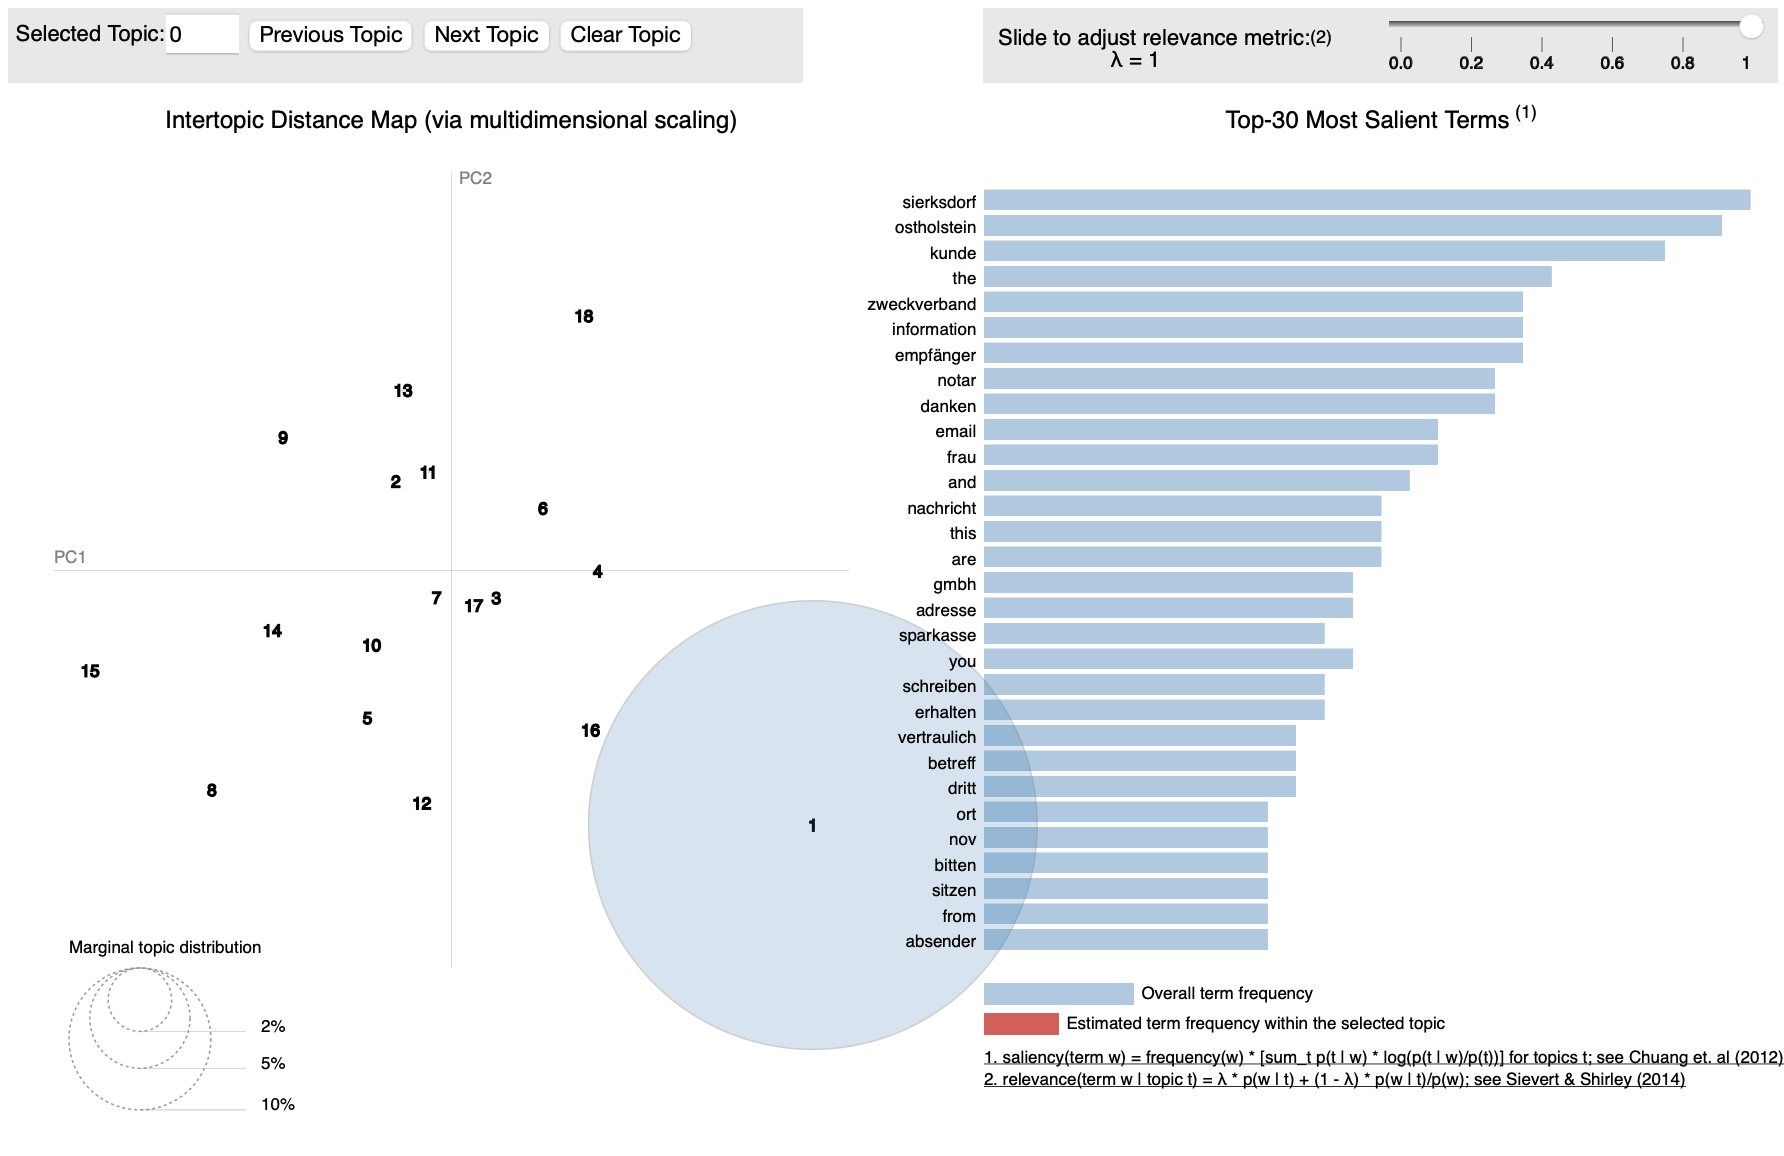
\includegraphics[scale=0.315]{lda_alpha001.png}
\end{center}
\caption{Je kleiner der $\alpha$-Wert wird, desto stärker dominiert ein Topic das Dokument.} 
\label{fig:img1}
\end{figure}\\
\begin{figure}[h]
\begin{center}
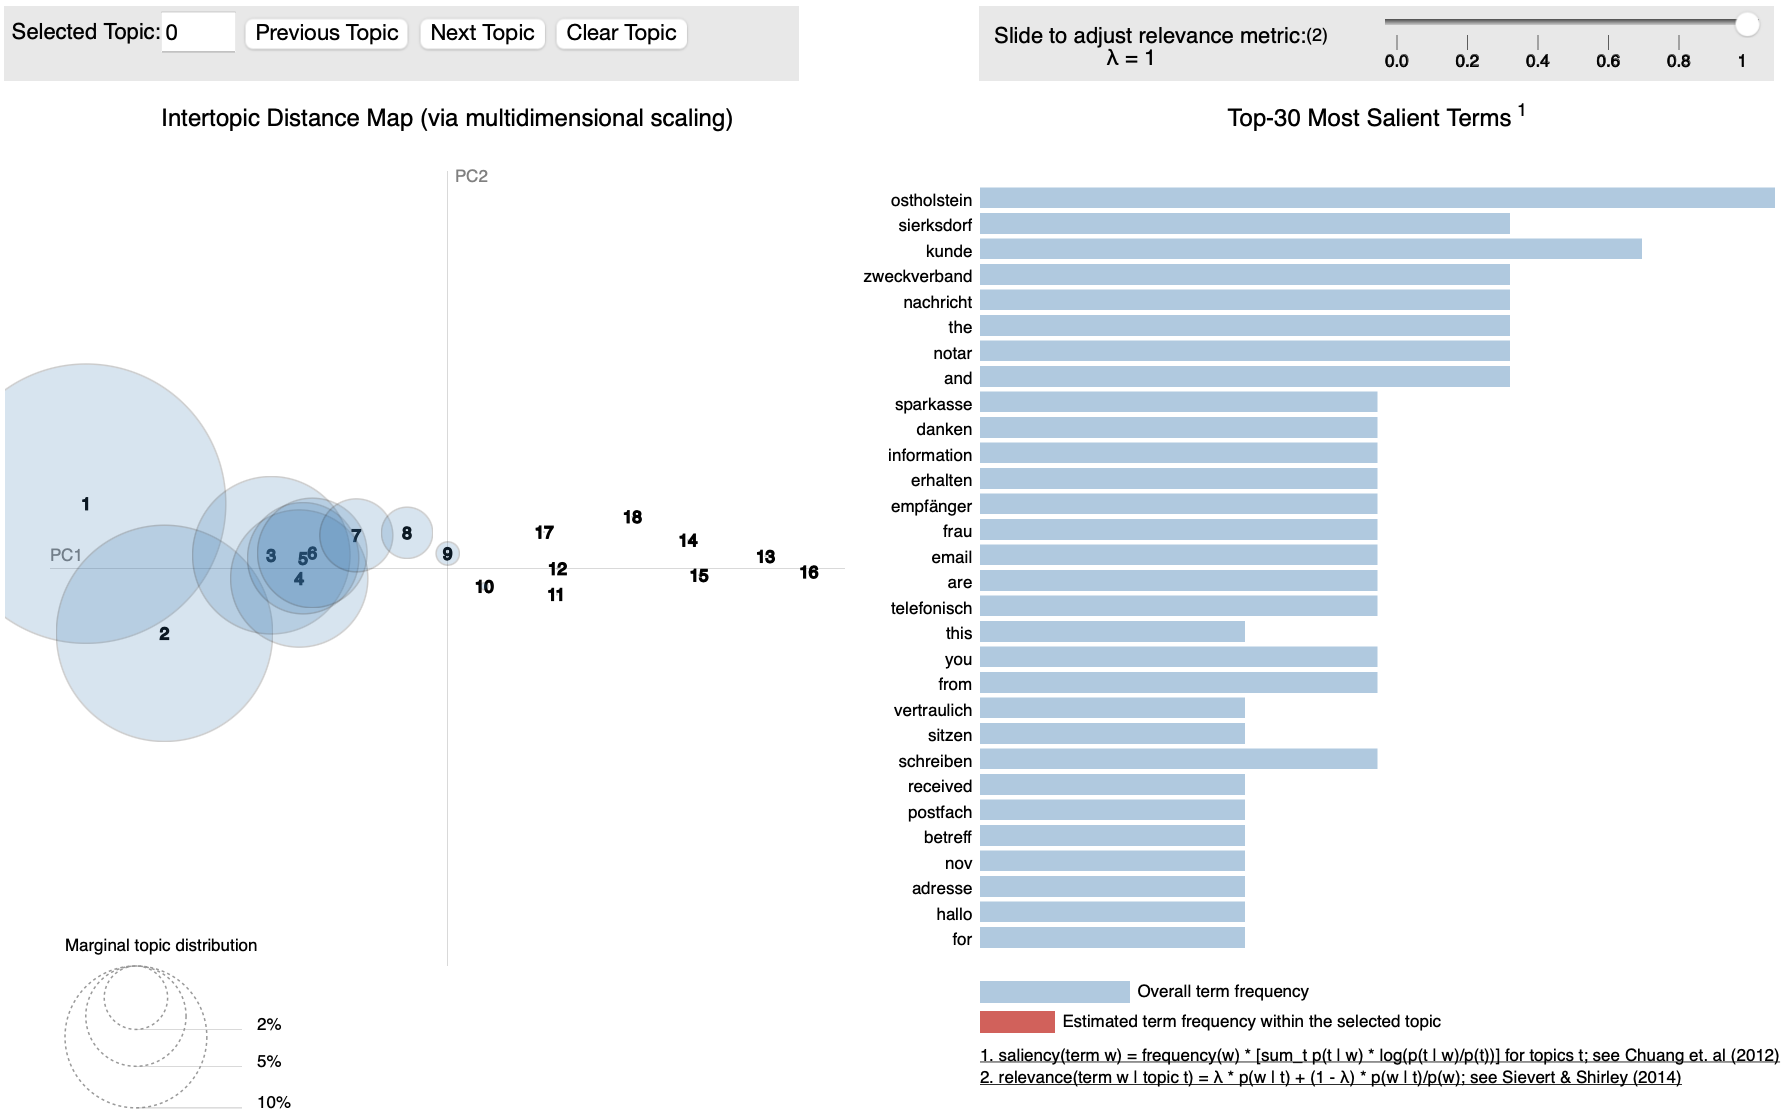
\includegraphics[scale=0.315]{lda_alpha1.png}
\caption{Je größer der $\alpha$-Wert wird, desto gleichmäßiger sind die Topics in dem Dokument beteiligt.}
\label{fig:img2}
\end{center}
\end{figure}\\
In der ersten Abbildung \ref{fig:img1} führt ein kleiner $\alpha = 0.01$ Wert zu einer sehr eindeutigen Dokument-Topic-Verteilung. Das erkennt man daran, dass es nur einen sehr großen blauen Kreis gibt. Jeder Kreis repräsentiert eine Topic und mit der Größe dessen Anteil am Dokument. Befinden sich zwei Kreise zum Teil auf der gleichen Position bedeutet das, dass sich die Wörter in den Topics zu einem gewissen Teil überschneiden. In Abbildung \ref{fig:img1} sind bei den meisten Topics nur die Zahlen und keine Kreise zu erkennen, da die Topics einen sehr kleinen Anteil an dem Dokument haben. Dies ist durch $\alpha$ bedingt. Bei der zweiten Abbildung \ref{fig:img2} hingegen haben wir ein $\alpha = 1$, was eine gleichmäßigere Verteilung zur Folge hat. So sieht man, dass es viele Kreise gibt, die sich zum Teil auch überlappen. Die Größe der Kreise unterscheidet sich nicht so stark voneinander, wie bei Abbildung \ref{fig:img1}, somit sind die Topics bezüglich ihren Anteils an dem Dokument ähnlicher zueinander. Der Trade-off zwischen den beiden Zielen ist der Grund für das Funktionieren von LDA, denn dadurch werden Gruppen mit semantisch eng miteinander verbundenen Wörtern, die oft miteinander vorkommen, gefunden. Nach dem gleichen Prinzip funktioniert die Dirichlet-Verteilung der Topic-Word-Verteilung $\beta$.  


\chapter{Konzeption} %%%%%%%%%%%%%%%%%%%%%%%%%%%%%%%%%%%%%%%%%%%%%%%%%%%%%%%%%%%%%%%%%KONZEPT

Dieser Abschnitt wird die Vorgehensweise beschreiben, wie unter der Nutzung der Daten der ZVO Topic-Modellierung umgesetzt wird, um Aufschluss über die Qualität der Daten zu erlangen. Dafür wird die Herangehensweise dargestellt und erklärt.

\section{Verfahrensweise}
Bei der ZVO sollen jährlich händisch aufgenommene Anfragen in Zukunft maschinell klassifiziert werden. Dafür wird im Rahmen des M4KK Projekts ein Kundenanfrage-Klassifikator erstellt. Für die korrekte Klassifikation ist die Qualität der vorliegenden Daten von hoher Bedeutung. Die Arbeit verfolgt das Ziel, die Qualität der Daten zu analysieren und semantische Gruppierungen zu analysieren. Dafür wird ein LDA Modell generiert, das als Datengrundlage alle verfügbaren ZVO Daten verwendet. Das Vorgehen ist wie folgt in Abbildung \ref{fig:flowchart} dargestellt:   

% FLOW CHART %%%%%%%
\tikzstyle{rect} = [rectangle, text centered, draw =black]
\tikzstyle{arrow} = [thick,->,>=stealth]
\begin{figure}[H]
\begin{center}
\begin{tikzpicture}[node distance = 2cm]
\node (mails) [rect] {Datenerhebung durch Mailanfragen};
\node (zuordnung) [rect, below of = mails] {Manuelle Zuordnung Daten zu Abteilungen};
\node (vorbereitung) [rect, below of = zuordnung] {Datenvorbereitung};
\node (LDA) [rect, below of= vorbereitung] {LDA Modell erstellen};
\node (Schluesselwoerter) [rect, below right of = LDA, node distance = 3cm]{Schlüsselwörter finden};
\node (Topics) [rect, below left of = LDA, node distance = 3cm] {Topics finden};
\node (Matrix) [rect, below of = Schluesselwoerter] {Matrix erstellen};
\node (Ueberschneidungen) [rect, below of = Matrix] {Überschneidungen analysieren};
\node (Topicsana)[rect, below of=Topics]{Topics und Keywords analysieren};
\draw [arrow] (mails) -- (zuordnung);
\draw [arrow] (zuordnung) -- (vorbereitung);
\draw [arrow] (vorbereitung) -- (LDA);
\draw [arrow] (LDA) -- (Schluesselwoerter);
\draw [arrow] (LDA) -- (Topics);
\draw [arrow] (Topics) -- (Topicsana);
\draw [arrow] (Schluesselwoerter) -- (Matrix);
\draw [arrow] (Matrix) -- (Ueberschneidungen);
\end{tikzpicture}
\caption{Prozessschritte von der Datenerhebung bis zur Analyse. Die Arbeit verfolgt zwei Ziele: Die Topicanalyse und Zuordnung von Topic und Label.}
\label{fig:flowchart}
\end{center}
\end{figure}

Nach der Erhebung der Daten können die einzelnen Anfragen manuell in die vorgegebenen Abteilungsgruppen eingeteilt werden. Dort wird die Datenreinigung vorgenommen. Sind die Daten bereinigt, kann das Feature Engineering beginnen, wonach die Daten für den Computer verständlich formatiert sind. Die Erstellung des LDA Modells wird vorgenommen, sobald der Korpus erstellt ist. Die Modellerstellung ist durch den in Abbildung \ref{fig:code1} gegebenen Pseudocode beschrieben. \\


\begin{figure}[h]
\begin{lstlisting}
data = " "
FOR d IN Anzahl Dokumente DO:
    data = data + str(d)
Teile data in einzelne items einer Liste auf
Erstelle ein Dictionary aus der Liste
Wandle ID aus Dictionary in Woerter um
Erstelle den Korpus
Erstelle das Modell
Gibt die Topic-Wort-Verteilungen für alle Topics aus
\end{lstlisting}	
\caption{Pseudoalgorithmus für die Prozesskette}
\label{fig:code1}
\end{figure}


Ist das Modell generiert und die Topics auslesbar, können die Daten evaluiert werden. Dazu werden zwei Ansätze verfolgt. Zum Einen werden Topics und zugehörigen Schlüsselwörter untersucht, um u.a. Aufschluss über mögliche Verbesserungspotentiale bei der Datenreinigung oder dem Feature Engineering festzustellen. Als zweites werden die vom Modell erfassten Gruppen betrachtet und den gegebenen manuell klassifizierten Abteilungen zugeordnet. Die folgenden Punkte beschreiben den Prozess im Detail: \\

%\begin{enumerate}
%\item \textbf{Gruppen und Wörter finden}\\
\subsection{Gruppen und Wörter finden}
Ein LDA Modell besteht aus zwei Verteilungen, die die zugrundeliegenden Daten semantisch darstellbar machen: die Dokument-Topic-Verteilung und die Topic-Word-Verteilung. Als Ausgabe des Modells ist also zu erkennen, welche Topics die Dokumentmenge durchschnittlich hauptsächlich beschreiben und welche Wörter in den Topics jeweils dominant vorkommen. Das Modell kann Topics nicht inhaltlich bennen, sondern nur die Verteilungen darstellen. Somit ist nicht eindeutig, welches Topic welche Abteilung der ZVO darstellt. Dafür betrachten wir die Topic-Word-Verteilungen und schließen von dieser auf die Qualität der Daten. Ist über die dominanten Wörter in einem Topic zu erkennen, welche Abteilung dieses repräsentiert, scheint das Modell und die Daten gut genug zu sein, um die Daten zu klassifizieren. Sollte die Abteilung nicht an den Wörtern ablesbar sein, sind die Daten nicht optimal für eine Klassifikation geeignet. Dabei ist auch relevant, wie oft die gleichen Wörter in den jeweiligen Topics vorkommen und ob Stop-Words Manipulation eine Option der Qualitätssteigerung darstellt.

%\item \textbf{Zuordnung Abteilung zu Topic}\\
\subsection{Zuordnung Abteilung zu Topic}
Das LDA Modell erstellt aus den Daten 18 Topics. Diese Topics sollten im optimalen Fall sehr ähnlich zu den händisch klassifizierten Abteilungen sein, wenn die vordefinierten Abteilungen eine akkurate Repräsentation der Topics in den Daten darstelle. Ist dies nicht der Fall, kann man auf eine schlechte Klassifikation schließen. Dies kann durch eine schlechte Qualität der Daten als auch durch eine ineffiziente manuelle Einteilung der Topics bedingt sein. Die Fähigkeit, Topics auf Abteilungen zu mappen, gibt Aufschluss über die Qualität der Daten. Für die Zuordnung werden zwei Matrizen verwendet: \lstinline{gruppen_LABEL} und \lstinline{gruppen_LDA}. Die erste sortiert alle Dokumentindizes als Listenelemente in die jeweilige Zeile der Matrix, sodass der Index eines händisch in Abteilung 3 eingeordneten Dokumentes in \lstinline{gruppen_LABEL[4]} zu finden ist. Die Verzögerung ergibt sich durch den ersten Listenindex $0$. Die Matrix \lstinline{gruppen_LDA} beinhaltet alle Indizes der Dokumente, die vom Modell klassifiziert wurden, in gleicher Struktur. Dafür wird für jedes Dokument, das den Korpus ausmacht, eine dokumentseigene Dokument-Topic-Verteilung errechnet. Das Topic, für das das Dokument am wahrscheinlichsten ist, bestimmt, welcher Teilliste der Dokumentindex angehängt wird. Beide Matrizen verfügen nun über die Indizes der Dokumente in den jeweiligen Topics bzw. Abteilungen und können anhand der einzigartigen Indizes auf Überschneidungen geprüft werden. Die Anzahl der Überschneidungen werden in einer Matrix gespeichert, die jedes Element von \lstinline{gruppen_LDA} auf jedes Element von \lstinline{gruppen_LABEL} abbildet und deren Überschneidung zählt. Eine optimale Zuordnung von Topic auf Abteilung ist möglich, wenn jede Zeile ein Maximum in einer Spalte hat, die nicht auch das Maximum einer anderen Zeile enthält. Ist dies jedoch nicht der Fall, sind die Daten in der aktuellen Form nicht optimal für die Klassifizierung. Dabei ist neben der Anzahl der Überschneidungen auch die die der Dokumente in dem Topic bzw. der Abteilung insgesamt als Vergleich relevant.Der Unterschied zwischen den beiden ist bei einer guten Klassifizierung klein. 
\end{enumerate}

\chapter{Implementierung}%%%%%%%%%%%%%%%%%%%%%%IMPLEMENTIERUNG
Dieser Abschnitt befasst sich mit der Implementierung des im Abschnitt 3 beschriebenen Konzepts. Dabei wird die Implementierung durch Python Code erklärt und die genaue Vorgehensweise dargestellt. Die Ergebnisse werden gezeigt, jedoch noch nicht analysiert. \\

Zur Untersuchung der Qualität der ZVO-Daten wird in dieser Arbeit die LDA Methode verwendet. Dabei wird nur der Text als bekannt angenommen. Die Topics sind zu Beginn nicht bekannt und sollen entdeckt werden. Als grundlegendes Topic-Modellierungs-Verfahren findet es Verwendung in einem breiten Anwendungsspektrum. Durch die Bekanntheit von LDA sind bereits viele Pakete und Bibliotheken in Programmierumgebungen vorzufinden und einfach zu implementieren. Seit LDAs Veröffentlichung in 2000 wurde eine umfassende und detailreiche Dokumentation entwickelt, die neben vielen Forenbeiträgen die Arbeit mit LDA stark erleichtern. Zusätzlich hat LDA in diesem Anwendungsfall den Vorteil, dass es nicht wie zum Beispiel LSA direkt Dokumentähnlichkeiten ausgibt, sondern das Ergebnis in Form einer Matrix darstellt, die Wörter auf Dokumente abbildet. Damit ergeben sich als Werte der Matrix die Topics, denen die Wörter jeweils angehören. Bei LDA Methoden ist die Anzahl der Topics ein individueller Input, durch den sich das Ergebnis schwerwiegend verändern kann. Die Werte in der Matrix können somit von $0$ bis zu der individuellen Anzahl der Topics reichen. Die optimale Anzahl an Topics ist grundsätzlich ein nicht einfaches Problem bei Anwendungen. Im Fall der ZVO werden als Anzahl der Topics 18  gewählt, da dies die Anzahl der bereits erstellten Abteilungen ist. \\

Bekannte Frameworks zur Topic-Modellierung implementieren grundsätzlich ähnliche Algorithmen. Betrachtet wurden in dieser Arbeit Mallet, Gensim und Sci-kit Learn.  Wichtige Schritte sind die Vorbereitung der Daten, die Implementierung, die Auswertung und die Visualisierung. Als Bibliothek wird in dieser Arbeit die Gensim Bibliothek verwendet, die für die Verarbeitung von unstrukturierten Daten und Anwendung von unüberwachten Algorithmen bekannt ist. Algorithmen, wie \lstinline{word2vec}, \lstinline{LSI} oder \lstinline{LDA} entdecken automatisch Strukturen durch das Prüfen von gemeinsam auftretenden Mustern im Korpus der Trainingsdaten. Viele bekannte Algorithmen sind bereits in diesem Framework implementiert, was die Umsetzung der Topic-Modellierung vereinfacht. Gensim erlangte in der Vergangenheit Bekanntheit durch seine hochoptimierten Implementierungen bekannter Algorithmen und der Schnelligkeit und Verlässlichkeit, mit der diese ausgeführt werden. Außerdem nutzt Gensim die Programmiersprache Python, was sich sehr gut für Probleme im Bereich des Data Science eignet. 


\section{Kundenanfragen des ZVO}
Die ZVO erhält jährlich viele digitale Anfragen von Kunden in Form von E-Mails. Die in dieser Arbeit verwendeten Daten sind eine Sammlung, die über mehrere Jahre erweitert wurde. Dabei wird jede E-Mail von einem Mitarbeiter der ZVO gelesen und in eine der 18 vordefinierten Abteilungen eingeteilt. In Zusammenarbeit mit der Universität zu Lübeck hat die ZVO 133045 unterschiedlich große Dokumente in Form einer XML Datei zur Verfügung gestellt. Die Daten wurden uni-intern zu einem Dataframe weiterverarbeitet. Die Daten wurden bereits formatiert und gereinigt, was somit nicht Teil dieser Arbeit ist. Das schließt unter anderem die Lemmatisierung und Entfernung von Stop-Words mit ein. Mittlerweile liegen sie in folgendem Format vor: 

\begin{figure}[h]
\begin{center}
\begin{tabular}{ccccccccc}
\hline
\hline
& filname & subject-message & Abt0 & Abt1 & Abt2 &  ... & Abt16 & Abt17\\
\hline
0 & FILE0& content0 &0&0&1&...&0&0\\
1& FILE1 & content1 &0 &0 &0 &... &1&0\\
2& FILE2 & content2 & 1 &0 &0 &...&0 &0 \\
3& FILE3 & content3 & 0 & 0 &1 &...&0 &1 \\
4& FILE4 & content4 & 0 & 1 &0 &...&1 &0 \\
...& ... & ... & ... & ...  &... &... &... & ... \\
133044& FILE133044 & content133044 & 0 &1 & 0&...&0&0\\
\hline
\hline
\end{tabular}
\caption{Die ZVO Daten liegen in einem Data Frame vor, der in subject-message die Kundenanfrage aus der Email speichert} 
\end{center}
\end{figure}

Relevant für die Auswertung sind die subject-message, die die eigentliche Anfrage enthält, und die jeweilige Abteilung, der sie von der ZVO händisch zugeordnet wurde. Die Tabelle verfügt über eine Matrix mit 18 Abteilungen, von denen pro subject-message eine oder mehrere mit einer 1 versehen ist bzw. sind. Dies beschreibt die Abteilung bzw. Abteilungen, der bzw. denen diese Anfrage manuell zugeordnet wurde. Die Daten in subject-message sind bereits bereinigt, also liegen wie in Abbildung \ref{fig:data1} vor:\\

\begin{figure}[h]
\begin{lstlisting}
OUTPUT: 
'wasser verbraucht amt deutschland ablesung zaehlen strom voll ort luebeck art straße messung verband nummer platz markieren wechsel lieferant stelle verbrauch kunde kunden anrede mann sommer beschwerde schrift allgemein kommunikation datenmanagement fern'
\end{lstlisting}
\caption{So könnte ein Datum der ZVO aussehen} 
\label{fig:data1}
\end{figure}\\

Um die Einträge in eine computer-lesbare Form zu verwandeln, muss ein Dictionary erstellt werden, das alle Wörter auf eine Anzahl ihrer Vorkommen abbildet. Dafür müssen die Wörter als alleinige Listeneinträge einlesbar sein, wie in Abbildung \ref{fig:data2}: \\

\begin{figure}[h]
\begin{lstlisting}
OUTPUT split: 
['wasser', 'verbraucht', 'amt', 'deutschland', 'ablesung', 'zaehlen', 'strom', 'voll', 'ort', 'luebeck', 'art', 'straße', 'messung', 'verband', 'nummer', 'platz', 'markieren', 'wechsel', 'lieferant', 'stelle', 'verbrauch', 'kunde', 'kunden', 'anrede', 'mann', 'sommer', 'beschwerde', 'schrift', 'allgemein', 'kommunikation', 'datenmanagement', 'fern']
\end{lstlisting}
\caption{Ein gesplittetes Datum vorbereitet für das Dictionary}
\label{fig:data2}
\end{figure}\\

\section{Datenvorbereitung}
Bevor die Topic-Modellierung auf den Daten durchgeführt werden kann, müssen die Daten einem Prozess unterzogen werden. Dieser beginnt mit der Datenakquise, also der Sammlung bestimmter relevanter Daten. Im Falle der ZVO bedeutet dies, dass es genügend Kundenanfragen gibt, die verarbeitet werden können. Wenn diese Daten bestehen, werden sie auf die relevanten Wörter reduziert, aus denen eine bedeutsame Inferenz von Informationen möglich ist, sodass unter anderem die sogenannten Stop-Words, also eine Menge von Wörtern, entfernt werden. Es gibt vordefinierte Sammlungen von Stop-Words und es können eigene definiert werden. Das Entfernen von Stop-Words verhindert, dass sich das Topic-Modell an den falschen Wörtern orientiert, die keine aussagekräftige semantische Information in sich tragen. Nachdem die Stop-Words entfernt wurden, ergeben die meisten Sätze keinen inhaltlichen Sinn mehr, wie in Abbildung \ref{fig:data1} zu erkennen. Dies ist jedoch nicht schlimm, da der nächste Schritt der Reinigung den Daten die Reihenfolge entzieht und das Bag of Words Modell erstellt. Dabei werden alle Wörter als eine Menge von unabhängigen Wörtern betrachtet, die sich nur durch ihre Vorkommensanzahl in dem Korpus unterscheiden. Dabei wird die Groß- und Kleinschreibung ebenfalls irrelevant, da es bei einer Menge von Wörtern ohne Reihenfolge auch keine Satzanfänge mehr gibt. Des weiteren besteht die Möglichkeit alle konjugierten bzw. deklinierten Formen eines Wortes zum Infinitiv bzw. Nominativ zusammenzufassen. Dies wird als Lemmatisierung bezeichnet. Wenn die Daten in der gewünschten Form vorliegen, beginnt der Schritt des Featureengineerings. Für einen Computer sind Wörter nicht so leicht zu verarbeiten, wie Zahlen, weshalb in diesem Schritt eine Quantisierung der Wörter und Überführung dieser in eine zahlenbasierte Form vorgenommen wird. Dabei sind die Features in Form der Spalten des Dataframes bereits passend gegliedert. Für die Darstellung der Dokumente als Menge an Zahlenwerten wird ein Dictionary erstellt, das die Wörter wie in Abbildung \ref{fig:data2} erhält und die Anzahl der Wörter ohne Duplikate in einer Liste auflistet. Diese Auflistung der Wörter zusammen mit ihrer Anzahl und laufenden Indexnummer kann als Input für ein LDA Modell verwendet werden. Die Worte werden intern als ID dargestellt, die für einen Menschen nicht zu verstehen sind. Aus diese Grund wird im Algorithmus der id2wordParameter eingeführt, der die Übersetzung zwischen Zahl und Datum darstellt. 

\section{Umsetzung Konzept}
Wie in Kapitel 3 beschrieben verfolgt die Arbeit zwei Ansätze. Im Folgenden wird die Umsetzung dieser dargelegt: \\
 
%\begin{enumerate}
%\item
\subsection{Gruppen und Wörter finden}
Alle Dokumente werden für die Erstellung eines Korpus genutzt. Der Korpus generiert eine Topic-Verteilung für die Gesamtheit aller Dokumente. Dabei werden zuerst alle Anfragedaten in einen String zusammengefügt, der als Grundlage für das Wörterbuch und den Korpus dient. Um diesen in ein Dictionary, also eine nummerierte Auflistung aller Wörter und dessen Anzahl, zu verwandelt, muss der String in eine Liste mit voneinander getrennten Items gesplittet werden. Hier wird ein Bag of Words Prinzip verfolgt, die Reihenfolge ist somit irrelevant für das Ergebnis des Modells. Aus der Liste wird dann das Dictionary erstellt. Durch den Aufruf des LDA Modells wird aus dem Bag of Words mithilfe des Dictionarys eine vorgegebene Anzahl an Topics aus der Wortenge modelliert, basierend auf häufig zusammen auftretenden Wörtern. Dadurch ergibt sich neben einer Verteilung der Topics in einem Modell die Verteilung der Wörter, die ein Topic besonders beeinflussen. Ist das Modell generiert, können die Topics ausgelesen werden. Der Programmcode für die beschreibenen Schritte ist in Abbildung \ref{fig:codeinput} dargestellt.\\
\\

\begin{figure}[H]
\begin{lstlisting}[language=Python, basicstyle=\small]
INPUT:
data = ''

# Zusammenfügen aller Dokumente in einen gorßen String
for x in range(0,106000):
    data += df.at[x,'subject-message']

# Aufteilen des Strings in viele einzelne Wörter
list = data.split()

# Erstellen eines Dictionarys
dictionary = corpora.Dictionary([list])
temp = dictionary[0]
id2word = dictionary.id2token

# Erstellen des Korpus
corpus = [dictionary.doc2bow(text) for text in [list]]

# Erstellen des LDA Modells
lda = LdaModel(corpus, num_topics=18, id2word = id2word)

#Ausgeben aller Topics inklusive Schlüsselwörtern
pprint(lda.print_topics())

\end{lstlisting}
\caption{Der Input zum Aufbau eines LDA Modells}
\label{fig:codeinput}
\end{figure}

Der Input-Code generiert aus allen Daten einen Korpus, der 18 Gruppen in den Daten findet. Jede Topic-Word-Verteilungen hat die Eigenschaft, alle Wörter des Korpus aufzulisten, auch wenn das Topic von gewissen Wörtern keinen Gebrauch macht. Die Topics, die von dem Modell generiert wurden, sind durch die 10 häufigsten Schlüsselwörter und ihren Wahrscheinlichkeiten zum Auftreten definiert. Der Output des in Abbildung \ref{fig:codeinput} definierten Algorithmus ist in Abbildung \ref{fig:codeoutput} gelistet. 

\begin{figure}[H]
\begin{lstlisting}[language=Python]
OUTPUT:
[(0,
  '0.012*"ostholstein" + 0.011*"nachricht" + 0.010*"sierksdorf" + '
  '0.009*"zweckverband" + 0.008*"betreff" + 0.008*"danken" + 0.007*"email" + '
  '0.007*"hra" + 0.007*"datum" + 0.007*"hyperlink"'),
 (1,
  '0.014*"ostholstein" + 0.011*"nachricht" + 0.010*"zweckverband" + '
  '0.009*"sierksdorf" + 0.008*"sitzen" + 0.008*"danken" + 0.007*"wagrienring" '
  '+ 0.007*"lübeck" + 0.007*"betreff" + 0.006*"the"'),
 (2,
  '0.014*"sierksdorf" + 0.013*"zweckverband" + 0.011*"nachricht" + '
  '0.010*"ostholstein" + 0.008*"danken" + 0.008*"betreff" + 0.007*"sitzen" + '
  '0.006*"the" + 0.006*"homepage" + 0.006*"frau"'),
  \end{lstlisting}
  \end{figure}
  \newpage
  \begin{figure}[h]
  \begin{lstlisting}
 (3,
  '0.014*"sierksdorf" + 0.011*"ostholstein" + 0.011*"nachricht" + '
  '0.010*"zweckverband" + 0.010*"betreff" + 0.008*"the" + 0.007*"frau" + '
  '0.006*"danken" + 0.006*"denken" + 0.006*"lübeck"'),
 (4,
  '0.012*"zweckverband" + 0.011*"frau" + 0.011*"sierksdorf" + '
  '0.011*"ostholstein" + 0.009*"nachricht" + 0.008*"betreff" + 0.007*"the" + '
  '0.007*"danken" + 0.006*"lübeck" + 0.006*"öffentlich"'),
 (5,
  '0.015*"zweckverband" + 0.011*"sierksdorf" + 0.011*"ostholstein" + '
  '0.009*"the" + 0.008*"betreff" + 0.007*"lübeck" + 0.007*"danken" + '
  '0.007*"nachricht" + 0.007*"hyperlink" + 0.006*"sitzen"'),
 (6,
  '0.013*"nachricht" + 0.012*"ostholstein" + 0.012*"zweckverband" + '
  '0.010*"betreff" + 0.009*"sierksdorf" + 0.007*"danken" + 0.006*"the" + '
  '0.006*"lübeck" + 0.006*"frau" + 0.005*"hyperlink"'),
 (7,
  '0.012*"ostholstein" + 0.012*"sierksdorf" + 0.011*"zweckverband" + '
  '0.010*"nachricht" + 0.008*"danken" + 0.008*"the" + 0.007*"hra" + '
  '0.007*"email" + 0.007*"betreff" + 0.006*"lübeck"'),
 (8,
  '0.012*"ostholstein" + 0.009*"sierksdorf" + 0.008*"nachricht" + '
  '0.008*"danken" + 0.008*"betreff" + 0.008*"frau" + 0.008*"zweckverband" + '
  '0.008*"hyperlink" + 0.007*"email" + 0.007*"homepage"'),
 (9,
  '0.013*"sierksdorf" + 0.012*"zweckverband" + 0.011*"ostholstein" + '
  '0.009*"nachricht" + 0.009*"danken" + 0.008*"frau" + 0.007*"the" + '
  '0.007*"lübeck" + 0.006*"hyperlink" + 0.006*"sitzen"'),
 (10,
  '0.011*"zweckverband" + 0.011*"nachricht" + 0.010*"sierksdorf" + '
  '0.010*"betreff" + 0.009*"ostholstein" + 0.009*"lübeck" + 0.007*"the" + '
  '0.007*"sitzen" + 0.007*"danken" + 0.007*"hyperlink"'),
 (11,
  '0.013*"sierksdorf" + 0.009*"ostholstein" + 0.009*"zweckverband" + '
  '0.008*"betreff" + 0.008*"nachricht" + 0.007*"danken" + 0.007*"hyperlink" + '
  '0.007*"lübeck" + 0.006*"email" + 0.006*"datum"'),
  \end{lstlisting}
  \end{figure}
  \newpage
  \begin{figure}[h]
  \begin{lstlisting}
 (12,
  '0.013*"ostholstein" + 0.012*"sierksdorf" + 0.009*"nachricht" + '
  '0.009*"zweckverband" + 0.008*"betreff" + 0.008*"danken" + 0.007*"email" + '
  '0.006*"frau" + 0.006*"lübeck" + 0.006*"wagrienring"'),
 (13,
  '0.013*"sierksdorf" + 0.010*"the" + 0.010*"zweckverband" + '
  '0.009*"ostholstein" + 0.009*"nachricht" + 0.008*"danken" + 0.007*"lübeck" + '
  '0.007*"betreff" + 0.007*"frau" + 0.007*"öffentlich"'),
 (14,
  '0.012*"zweckverband" + 0.011*"danken" + 0.011*"sierksdorf" + '
  '0.010*"ostholstein" + 0.010*"betreff" + 0.008*"nachricht" + '
  '0.007*"hyperlink" + 0.007*"gmbh" + 0.006*"lübeck" + 0.006*"kundennummer"'),
 (15,
  '0.014*"ostholstein" + 0.011*"sierksdorf" + 0.008*"zweckverband" + '
  '0.008*"danken" + 0.008*"frau" + 0.007*"betreff" + 0.007*"the" + '
  '0.007*"nachricht" + 0.006*"amtsgericht" + 0.006*"sitzen"'),
 (16,
  '0.014*"zweckverband" + 0.013*"ostholstein" + 0.011*"nachricht" + '
  '0.009*"danken" + 0.008*"sierksdorf" + 0.007*"hyperlink" + 0.007*"lübeck" + '
  '0.006*"sitzen" + 0.006*"the" + 0.006*"betreff"'),
 (17,
  '0.012*"ostholstein" + 0.011*"danken" + 0.011*"sierksdorf" + 0.009*"betreff" '
  '+ 0.009*"zweckverband" + 0.008*"nachricht" + 0.007*"the" + 0.007*"frau" + '
  '0.006*"hyperlink" + 0.006*"sitzen"')]
\end{lstlisting}
\caption{Die Topics und Schlüsselwörter}
\label{fig:codeoutput}
\end{figure}

Das LDA hat erfolgreich auf allen verfügbaren Daten ein Modell gebaut, das die Daten in Topics $[0,17]$ eingeteilt hat. Jedes Topic hat dominante Wörter, die zusammen mit ihren jeweiligen Auftretenswahrscheinlichkeiten aufgeslistet sind. Dabei sind dies nur die Wörter mit der höchsten Vorkommenswahrscheinlichkeit. Jedes Topic wird von allen verfügbaren Wörtern im Dictionary dargestellt, nur zu einem unterschiedlichen Anteil. Die Wahrscheinlichkeiten für das Auftreten von Wörtern liegt im Intervall $[1.5\%,0\%]$. Dabei sind viele Wörter in mehreren Topics als Schlüsselwörter zu finden. \\


\subsection{Zuordnung Abteilung zu Topic}
Die Qualität der Daten und des Klassifikators kann alternativ über die Zuordnung der Topics zu den Abteilungen untersucht werden. Die optimalen Daten werden eine perfekte Zuordnung schaffen, ohne beim Modell eine Verwirrung festzustellen. Dafür wird in dieser Arbeit untersucht, wie gut sich die Topics auf die Abteilungen zuordnen lassen. Der wohl naivste Ansatz ist, Topic $x$ auf Abteilung $x$ für alle $x \in [0,17]$ abzubilden. Dafür ist die Anzahl der Dokumente pro Topic bzw. Abteilung relevant. Dabei wird nur die Anzahl der zugeordneten Dokumente überprüft, indem für jedes auf Basis des Korpus eine Dokument-Topic-Verteilung generiert wird. Bei dieser wird vom Algorithmus die Topic, für die die höchste Wahrscheinlichkeit errechnet wurde, für das Dokument ausgewählt. Um welche Dokumente es sich jedoch bei dem Vergleich jeweils tatsächlich handelt ist zu diesem Punkt noch irrelevant. Überschneidungen werden noch nicht betrachtet. In Abbildung \ref{fig:count1} ist die Anzahl der Dokumente in den Topics dargestellt:

\begin{figure}[H]
\begin{center}
\begin{tabular}{cc}
\hline 
\hline
Topic&Counts LDA\\
\hline
T0&8605\\
T1&3959\\
T2&5974\\
T3&1714\\
T4&5823\\
T5&2291\\
T6&23558\\
T7&12721\\
T8&4207\\
T9&1100\\
T10&10021\\
T11&3243\\
T12&14556\\
T13&2697\\
T14&29456\\
T15&1162\\
T16&575\\
T17&1400\\
\hline
\hline
\end{tabular}
\caption{Anzahl Dokumente in den Topics}
\label{fig:count1}
\end{center}
\end{figure}
\\
Dasselbe ergibt sich für die Abteilungen und die Anzahl derer Dokumente. Dafür wird in dem von der ZVO bereitgestellten Datensatz die Zuordnung für jedes Dokument abgefragt. Dadurch kann das Dokument akkurat der Topic zugewiesen werden, wie es händisch getan wurde. Dies ist in Abbildung \ref{fig:count2} zu erkennen. \\ 

\begin{figure}[H]
\begin{center}
\begin{tabular}{cc}
\hline
\hline
Abteilung & Counts Label\\
\hline
L0&9770\\
L1&21061\\
L2&14245\\
L3&235\\
L4&1307\\
L5&251\\
L6&4009\\
L7&3610\\
L8&9410\\
L9&23533\\
L10&20676\\
L11&43\\
L12&2866\\
L13&9616\\
L14&8144\\
L15&12126\\
L16&4748\\
L17&2700\\
\hline
\hline
\end{tabular}
\caption{Anzahl Dokumente in den Abteilungen}
\label{fig:count2}
\end{center}
\end{figure}

Bei diesem Ansatz muss bedacht werden, dass ein Dokument von der ZVO in mehrere Abteilungen eingeteilt werden kann, während der Algorithmus in diesem Fall das Dokument immer nur einem Topic zuordnen. Da die Mehrheit der Dokument jedoch nur einer Abteilung zugewiesen ist, entsteht hier nur eine kleine Tendenz, die die Daten der ZVO in Abbildung \ref{fig:count2} etwas mehr Dokumente zuordnet, als in Abbildung \ref{fig:count1}.\\

In Abbildung \ref{fig:count2} sind die Abteilungen über Labels von $0$ bis $17$ aufgelistet. Dabei dient der Begriff Label der Adressierung einer Abteilung. So stellt Label 0 die Abteilung 0 der ZVO dar. Im Anwendungsfall steht jedes Label damit für eine reale Abteilung. Die Zuordnung der Labels zu Abteilungen ist in Tabelle \ref{fig:labels} dargestellt.


\begin{figure}[h]
\begin{center}
\begin{tabular}{ll}
\hline
\hline
Label&Abteilung\\
\hline
L0&Ablesung\\
L1&Allgemeiner Schriftverkehr\\
L2&BM-Beschwerden\\
L3&KA-Kommunaler Ausfall\\
L4&MaKo-Klärfälle\\
L5&ZSB-Aktionen\\
L6&ZSB-BAV\\
L7&ZSB-Zählerdatenmanagement\\
L8&ZSC-Forderungsmanagement\\
L9&ZSK-An/Abmeldungen\\
L10&ZSK-Bank\\
L11&ZSK-Interessenten\\
L12&ZSK-Korrekturrechnungen\\
L13&ZSK-Schwierige Fälle\\
L14&ZSK-Stammdaten/Postrückläufer\\
L15&ZSK-Standard Abfall\\
L16&ZSK-Standard Verbrauch\\
L17&ZSK-Widersprüche Abfall\\
\hline
\hline
\end{tabular}
\caption{Die Zuordnung von Label zu Abteilung}
\label{fig:labels}
\end{center}
\end{figure}\\


Die Anzahl der Dokumente eines Topics kann nun mit der einer Abteilung verglichen werden, um die grundsätzliche Kompatibilität zwischen Topics und Abteilungen prüfen zu können. Dies gibt jedoch nur eine grobe Richtung an, da die Dokument selbst nicht geprüft werden. Das bedeutet, dass die verglichenen Anzahlen nicht prüfen, ob es sich sowohl in der Topic, als auch in der Abteilung auch wirklich um das gleiche Dokument handelt. Um die Dokumente mit in den Vergleich einzubeziehen und damit die Zuordnung von Topic auf Abteilung zu verbessern, wird eine weitere Methode betrachtet. Die Zuordnung der Topics zu Abteilungen kann approximiert werden, indem gezählt wird, in wie vielen Dokumenten sich die Topics und Abteilungen jeweils überschneiden. Genau wie bei der Gruppeneinteilung wird für diese Überschneidung jedes Dokument erneut auf dem Korpus geprüft, um dessen Topic-Wort-Verteilung zu erstellen. Die Dokumente werden anhand ihrer einzigartigen Zeilen-ID adressiert. Die IDs werden der Topic zugeordnet, die die höchste Wahrscheinlichkeit in der Verteilung des Dokuments erreicht. Die Zuordnung findet in einer großen Liste statt, die über 18 Unterlisten verfügt, in die die IDs jeweils hinzugefügt werden. Die Überschneidungen werden in einer Matrix dargestellt, die für jedes Topic des Modells die Überschneidungen zu jeder Abteilung auflistet. Somit kann für jede Zeile die passende Zuordnung gefunden werden. Dabei stellt eine Zeile jeweils die Dokumente dar, die aufsummiert die Zahl einer Zeile in Abbildung \ref{fig:count1} ergeben. 

%comp bei 10000: [[536, 91, 67, 1, 12, 1, 12, 6, 23, 145, 69, 0, 22, 12, 38, 87, 24, 6], [15, 22, 11, 0, 2, 0, 0, 1, 7, 32, 77, 0, 6, 3, 5, 16, 3, 1], [6, 50, 81, 1, 3, 1, 31, 6, 28, 61, 30, 0, 18, 15, 22, 33, 4, 16], [14, 69, 58, 3, 3, 0, 19, 11, 37, 104, 63, 0, 18, 20, 21, 51, 33, 5], [7, 81, 104, 1, 3, 0, 7, 9, 56, 112, 97, 1, 11, 28, 36, 42, 15, 12], [0, 4, 3, 1, 0, 0, 1, 0, 2, 5, 3, 0, 1, 1, 0, 1, 0, 0], [2, 7, 24, 0, 0, 0, 2, 0, 7, 25, 23, 0, 2, 5, 2, 13, 8, 1], [19, 331, 90, 3, 16, 3, 49, 22, 111, 206, 200, 2, 29, 49, 61, 127, 36, 44], [3, 20, 33, 0, 1, 0, 2, 1, 11, 41, 78, 0, 3, 5, 7, 15, 8, 1], [4, 21, 17, 0, 2, 0, 1, 2, 26, 18, 33, 0, 3, 9, 5, 4, 2, 0], [13, 137, 115, 0, 6, 0, 25, 16, 53, 183, 136, 3, 6, 34, 75, 57, 39, 9], [27, 429, 221, 8, 34, 4, 129, 34, 291, 312, 271, 2, 48, 137, 75, 149, 50, 106], [0, 12, 8, 0, 1, 0, 3, 2, 5, 24, 13, 0, 2, 1, 3, 10, 5, 1], [12, 89, 73, 0, 9, 1, 9, 18, 25, 106, 124, 0, 4, 14, 29, 69, 52, 5], [10, 174, 110, 4, 11, 1, 15, 5, 42, 226, 137, 1, 19, 38, 39, 181, 21, 27], [8, 67, 70, 1, 4, 0, 11, 4, 21, 85, 115, 0, 8, 16, 20, 47, 21, 14], [19, 33, 44, 0, 5, 0, 4, 4, 18, 56, 63, 0, 6, 9, 16, 18, 7, 3], [39, 47, 52, 0, 5, 1, 15, 10, 203, 74, 71, 1, 12, 13, 16, 33, 17, 6]]

\begin{figure}[H]
\begin{center}
\tiny
\renewcommand{\arraystretch}{2}
\begin{tabular}{ccccccccccccccccccc}
\hline
\hline 
&L0&L1&L2&L3&L4&L5&L6&L7&L8&L9&L10&L11&L12&L13&L14&L15&L16&L17\\
\hline
\hline
T0&555& 977& \textbf{2150}& 21& 66& 19& 211& 251& 910& 960& 902& 2& 210& 596& 302& 758& 318& 250\\
\hline 
T1&512& 580& \textbf{650}& 3& 36& 7& 139& 101& 370& 453& 570& 0& 66& 378& 91& 196& 123& 53\\
\hline 
T2&508& 755& 263& 9& 67& 21& 254& 145& 282& \textbf{1498}& 1207& 1& 119& 300& 479& 527& 177& 130\\
\hline 
T3&108& 179& 98& 2& 15& 3& 33& 57& 236& \textbf{432}& 218& 0& 34& 55& 153& 198& 74& 27\\
\hline 
T4&493& 867& 442& 5& 63& 8& 134& 180& 451& \textbf{1111}& 1033& 8& 73& 348& 446& 489& 191& 89\\
\hline 
T5&91& 467& 98& 5& 25& 2& 60& 75& 162& \textbf{480}& 309& 1& 55& 127& 169& 351& 113& 47\\
\hline 
T6&1263& 3993& 1738& 28& 127& 48& 811& 587& 1384& 4139& \textbf{4730}& 6& 573& 2096& 1620& 2080& 680& 495\\
\hline 
T7&\textbf{3376}& 1298& 870& 17& 524& 16& 221& 338& 662& 1904& 1740& 9& 185& 381& 664& 891& 537& 133\\
\hline 
T8&310& 585& 216& 10& 27& 5& 67& 114& 203& 771 & \textbf{1013}& 0& 81& 323& 264& 440& 205& 73\\
\hline 
T9&58& 126& 47& 0& 3& 1& 17& 16& 131& 174& \textbf{400}& 0& 15& 55& 63& 69& 59& 17\\
\hline 
T10&286& \textbf{1610}& 1733& 12& 51& 27& 284& 299& 858& 1567& 1331& 4& 239& 893& 674& 673& 304& 248\\
\hline 
T11&194& 409& 377& 8& 27& 3& 88& 122& 180& \textbf{678}& 470& 0& 80& 173& 167& 395& 142& 118\\
\hline 
T12&486& 2355& 2495& 16& 80& 24& 564& 327& 1005& \textbf{2672}& 1513& 3& 311& 1254& 886& 1377& 579& 327\\
\hline 
T13&151& 393& 198& 5& 23& 4& 64& 83& 160& 414& \textbf{639}& 1& 68& 192& 123& 275& 151& 68\\
\hline 
T14&1008& 6084& 2681& 86& 153& 61& 990& 820& 2223& \textbf{5730}& 3832& 8& 701& 2327& 1860& 3093& 993& 552\\
\hline 
T15&270& 95& 36& 3& 10& 1& 29& 32& 46& 228& \textbf{284}& 0& 19& 31& 61& 81& 23& 21\\
\hline 
T16&81& 82& 25& 1& 3& 0& 18& 38& 27& \textbf{105}& 90& 0& 14& 29& 37& 76& 24& 15\\
\hline
T17&20& 206& 128& 4& 7& 1& 25& 25& 120& \textbf{217}& 395& 0& 23& 58& 85& 157& 55& 37\\
\hline
\hline
\end{tabular}
\caption{Anzahl der Überschneidungen zwischen LDA Topics (vert.) und ZVO Labels (horiz.) mit den maximalen Werten pro Zeile in \textbf{fett} markiert.}
\label{fig:matrixnormal}
\end{center}
\end{figure}\\


%[[555, 977, 2150, 21, 66, 19, 211, 251, 910, 960, 902, 2, 210, 596, 302, 758, 318, 250], [512, 580, 650, 3, 36, 7, 139, 101, 370, 453, 570, 0, 66, 378, 91, 196, 123, 53], [508, 755, 263, 9, 67, 21, 254, 145, 282, 1498, 1207, 1, 119, 300, 479, 527, 177, 130], [108, 179, 98, 2, 15, 3, 33, 57, 236, 432, 218, 0, 34, 55, 153, 198, 74, 27], [493, 867, 442, 5, 63, 8, 134, 180, 451, 1111, 1033, 8, 73, 348, 446, 489, 191, 89], [91, 467, 98, 5, 25, 2, 60, 75, 162, 480, 309, 1, 55, 127, 169, 351, 113, 47], [1263, 3993, 1738, 28, 127, 48, 811, 587, 1384, 4139, 4730, 6, 573, 2096, 1620, 2080, 680, 495], [3376, 1298, 870, 17, 524, 16, 221, 338, 662, 1904, 1740, 9, 185, 381, 664, 891, 537, 133], [310, 585, 216, 10, 27, 5, 67, 114, 203, 771, 1013, 0, 81, 323, 264, 440, 205, 73], [58, 126, 47, 0, 3, 1, 17, 16, 131, 174, 400, 0, 15, 55, 63, 69, 59, 17], [286, 1610, 1733, 12, 51, 27, 284, 299, 858, 1567, 1331, 4, 239, 893, 674, 673, 304, 248], [194, 409, 377, 8, 27, 3, 88, 122, 180, 678, 470, 0, 80, 173, 167, 395, 142, 118], [486, 2355, 2495, 16, 80, 24, 564, 327, 1005, 2672, 1513, 3, 311, 1254, 886, 1377, 579, 327], [151, 393, 198, 5, 23, 4, 64, 83, 160, 414, 639, 1, 68, 192, 123, 275, 151, 68], [1008, 6084, 2681, 86, 153, 61, 990, 820, 2223, 5730, 3832, 8, 701, 2327, 1860, 3093, 993, 552], [270, 95, 36, 3, 10, 1, 29, 32, 46, 228, 284, 0, 19, 31, 61, 81, 23, 21], [81, 82, 25, 1, 3, 0, 18, 38, 27, 105, 90, 0, 14, 29, 37, 76, 24, 15], [20, 206, 128, 4, 7, 1, 25, 25, 120, 217, 395, 0, 23, 58, 85, 157, 55, 37]] MIT 133044 Dokumenten!!!!

Diese Matrix bildet die Überschneidungen aller 133044 Dokumenten ab. Dabei sind die 18 LDA Topics auf der vertikalen Achse und die 18 LABEL Abteilungen auf der horizontalen Achse aufgetragen. Bezüglich der Zuordnung ist der naivste Ansatz, jeder Zeile (also LDA Topic) die Spalte (also Label Abteilung) mit der maximalen Überschneidung zuzuordnen. Dabei ist das Ziel die Anzahl der Gesamtüberschneidungen zu maximieren. \\


%\end{enumerate}

	
\chapter{Experimentelle Evaluation und Analyse}%%%%%%%%%%%%%%%%%%%%%%%%%%%%%%%%%%%%%%%%%%%%%%%%%%%%%%%%%ANALYSE
Die Implementierung des LDA Modells wurde im vorausgegangenen Teil vorgenommen. In diesem Abschnitt werden die Ausgaben analysiert und aus verschiedenen Perspektiven auf Erkenntnisse geprüft. Wie in Abschnitt 3 und 4 wird auch dieser Abschnitt in die zwei Teilbereiche dieser Arbeit unterteilt.\\

%\begin{enumerate}
%\item 
\subsection{Gruppen und Wörter finden}\\
Das LDA Modell hat 18 Gruppen aus den Daten generiert und diese mit einer Verteilung von Schlüsselwörtern beschrieben. Als Anwendungsziel in Bezug auf die ZVO sollen die Topics des Modells in Zukunft die Abteilungen darstellen. Betrachtet man dafür die Wörter der Topics, um die Topics semantisch den Abteilungen zuzuordnen, wird dies nicht gelingen. Das liegt daran, dass sich die dominaten Wörter in den Topics zu stark überschneiden. Zum Beispiel gehört ostholstein in allen Topics zu den häufigsten 5 Wörtern. In der folgenden Darstellung sind die häufigsten 5 Wörter aufgelistet und mit den 18 Topics auf Vorkommen geprüft: 

\begin{figure}[H]
\begin{center}
%\tiny
%\renewcommand{\arraystretch}{2}
%\begin{tabular}{ccccccccccccccccccc}
%Wort&L0&L1&L2&L3&L4&L5&L6&L7&L8&L9&L10&L11&L12&L13&L14&L15&L16&L17&L18\\
\begin{tikzpicture}
  \begin{axis}[title  = Topicabdeckung der häufigsten 5 Schlüsselwörter,
    xbar,
    y axis line style = { opacity = 0 },
    axis x line       = none,
    tickwidth         = 0pt,
    ytick             = data,
    enlarge y limits  = 0.05,
    enlarge x limits  = 0.02,
    width=0.7\textwidth,,
    bar width=5.5mm,    symbolic y coords = {oosthosltein,sierksdorf,zweckverband,nachricht,betreff,danken,frau,the,sitzen}, nodes near coords
  ]
  \addplot coordinates { (18,ostholstein)(17,zweckverband)(18,sierksdorf)(14,nachricht)(10,betreff)(8,danken)(2,frau)(2,the)(1,sitzen)};
  \end{axis}
\end{tikzpicture}
\caption{Topicabdeckung der häufigsten 5 Wörter aller Topics}
\label{fig:top5}
\end{center}
\end{figure}

In Abbildung \ref{fig:top5} sind die häufigsten 5 Wörter aller Topics auf der Y-Achse aufgelistet. Die X-Achse beschreibt die Anzahl der Topics, die das bestimmte Wort als eines der häufigsten 5 besitzen. Hätten alle 18 Topics Schlüsselwörter, die das Topic eindeutig beschreiben, würden sich 90 verschiedene Wörter auf der Y-Achse ergeben. Hier sind jedoch nur 9 Wörter aufgezählt, deren Anzahl sich auf 90 addiert. Die Topics teilen sich also auf 90 möglichen Schlüsselwörtern nur 9 Stück. Das bedeutet, dass sich die Topics semantisch sehr schwach bis garnicht von einander unterscheiden lassen. Dies ist auf die Qualität der Daten und dessen Wörter zurückzuführen. Die Topics lassen sich nicht stark genug von einander abgrenzen, wenn in jeden Topic die selben Wörter zu einem hohen Anteil vorkommen. Somit kann die Qualität der Daten und damit die des Klassifikators erhöht werden, indem die Stoppwörter erweitert werden. Wenn man beispielsweise das Wort ostholstein betrachtet, ist dies nicht aussagekräftig für die Abteilung, da sich alle Abteilungen in Ostholstein befinden. Die Wahl der zu ergänzenden Stoppwörter hängt also mit von der semantischen Bedeutung des Wortes ab. Dazu muss auf die Anzahl der Wörter insgesamt geachtete werden und die stark vertretenen Worte dieser Art entfernt werden. Zuletzt ist bedeutend, wie stark die semantische Bedeutung des jeweiligen Wortes für die bestimmte Abteilung ist. Ein Wort, das eine ganz bestimmt Abteilung beschreibt, wie ablesen die Abteilung Ablesung, darf dies natürlich nicht entfernt werden. 
\\

%\item 
\subsection{Zuordnung Abteilung zu Topic}\\
%Die durchschnittliche Überschneidung zwischen Abteilung und Topic spiegelt wieder, wie stark die Abteilung mit einem oder mehreren Topics übereinstimmt. Ein hoher Durschnitt kann entweder eine sehr hohe Überschneidung der Abteilung mit einer Topic oder relativ hohe Überschneidungen mit mehreren Topics bedeuten. Für die Umsetzung betrachten wir die Abbildung \ref{fig:matrixnormal} aus Abschnitt 4, die eine Matrix mit allen Überschneidungen zwischen Topics und Abteilungen mit absoluten Werten aufzeichnet. Hierbei beinhalten die Werte nur Dokumente, die sowohl in der Topic, als auch in der Abteilung enthalten sind. Um eine möglichst effektive Zuteilung zu erlangen, wählen wir zuerst den naivsten Ansatz, aus jeder Zeile den maximalen Wert zu nehmen. Als Graphik ist das wie folgt darzustellen: 
Wie in der Konzeption beschrieben ist der naivste Ansatz, um die Topics als Abteilungen zu interpretieren, den Topics der Reihenfolge nach die Abteilungen zuzuordnen. Also würde Topic 0 Abteilung 0 zugeteilt bekommen. \\
%\begin{figure}[H]
\begin{center}
\begin{tikzpicture} 
\begin{axis} [tick label style={/pgf/number format/fixed}, scaled ticks=false,ybar,xmin=-1,xmax=18,ymin=0,ymax=30000, bar width=8pt, height=8cm,width=15cm, ylabel={Anzahl Elemente}, xlabel={Topics bzw. Abteilungen}]
\addplot coordinates {
    (0,8605)
    (1,3959)
    (2,5974)
    (3,1714)
    (4,5823)
    (5,2291)
    (6,3558)
    (7,12721)
    (8,4207)
    (9,1100)
    (10,10021)
    (11,3243)
    (12,14556)
    (13,2697)
    (14,29456)
    (15,1162)
    (16,575)
    (17,1400)
};
\addplot coordinates {
(0,9770)
(1,21061)
(2,14245)
(3,235)
(4,1307)
(5,251)
(6,4009)
(7,3610)
(8,9410)
(9,23533)
(10,20676)
(11,43)
(12,2866)
(13,9616)
(14,8144)
(15,12126)
(16,4748)
(17,2700)
};
\legend{LDA, Label};
\end{axis}
\caption{Vergleich der Anzahl an Dokumenten pro Topic bzw. Abteilung}
\label{fig:countschart}
\end{tikzpicture}
\end{center}
%\end{figure}

Das Säulendiagramm in Abbildung \ref{fig:countschart} bildet jeweils für alle $x \in [0,17]$ Abteilung x auf Topic x ab und stellt die Anzahl in diesen Topics bzw. Abteilungen gegenüber. Dies zeigt, dass die Topics nicht optimal auf die Abteilungen abgebildet sind. Die Anzahl der enthaltenen Dokumente sollte ähnlicher sein. Betrachtet man zum Beispiel Topic 14, kann diese nicht Abteilung 14 darstellen, da es sich um einen Unterschied von 21312 Dokumenten, also 72$\%$, handelt.\\

Die Abbilung \ref{fig:countchart} zeigt, dass die Topics unabhängig von ihrem Index jedem Topic zugeordnet werden könnten. Um die korrekte Zuordnung zu finden, müssen alternative Ansätze gefunden werden. In den Abbildungen \ref{fig:count1} und \ref{fig:count2} ist die Anzahl der Dokumente in den jeweiligen Topics und Abteilungen aufgelistet. Um eine bessere Übersicht über die Daten zu bekommen, sind die Listen in den folgenden Abbildungen nach der Größe sortiert und mit einem weiteren Parameter dargestellt, der als Vergleichswert dienen soll. Dieser Parameter stellt den prozentualen Anteil der Topics im Korpus dar: 

\begin{figure}[H]
\begin{center}
\begin{tabular}{ccc}
\hline 
\hline
Topics & Counts LDA & Anteil$[\%]$\\
\hline
14&29456&22.13\\
6&23558&17.7\\
12&14556&10.94\\
7&12721&9.56\\
10&10021&7.53\\
0&8605&6.47\\
2&5974&4.49\\
4&5823&4,38\\
8&4207&3.16\\
1&3959&2.98\\
11&3243&2.44\\
13&2697&2.03\\
5&2291&1.72\\
3&1714&1.29\\
17&1400&1.05\\
15&1162&0.87\\
9&1100&0.83\\
16&575&0.43\\
\hline
\hline
\end{tabular}
\caption{Anzahl Dokumente in Topics mit relativem Anteil}
\label{fig:count3}
\end{center}
\end{figure}

%\quad

\begin{figure}[H]
\begin{center}
\begin{tabular}{ccc}
\hline
\hline
Abteilung & Counts Label & Anteil$[\%]$\\
\hline
9&23533&15.86\\
1&21061&14.20\\
10&20676&13.94\\
2&14245&9.6\\
15&12126&8.17\\
0&9770&6.59\\
13&9616&6.48\\
8&9410&6.34\\
14&8144&5.49\\
16&4748&3.20\\
6&4009&2.7\\
7&3610&2.43\\
12&2866&1.93\\
17&2700&1.82\\
4&1307&0.88\\
5&251& 0.17\\
3&235&0.16\\
11&43&0.03\\
\hline
\hline
\end{tabular}
\caption{Anzahl Dokumente in Abteilungen mit relativem Anteil}
\label{fig:count4}
\end{center}
\end{figure}


Nun wird durch die quantitativere Darstellung deutlich, dass sich nicht alle Topics eindeutig einer Abteilung zuordnen lassen. Dafür sind die Anzahlen in Abbildung \ref{fig:count3} und Abbildung \ref{fig:count4} zu unterschiedlich. Das Ergebnis zeigt, dass die Topic-Verteilung bei LDA das 14. Thema stärker erkennt, als die ZVO die Abteilung mit den meisten zugeordneten Dokumenten. Diese unterschieden sich durch $5923$ Dokumente. Die Betrachtung der unterschiedlichen Anteile dient somit nicht gut als Zuordnungsmethode, kann jedoch Aufschluss darüber geben, dass die Daten von der ZVO gleichmäßiger zugeteilt wurden, als sie von dem Topic-Modell erkannt werden. Dies bedeutet, dass die Wörter in den Dokumenten in ihrer Bedeutung und syntaktischen Umgebung zu ähnlich sind, als dass sie sich optimal in die von der ZVO vorgegebenen Abteilungen einteilen lassen. Dies könnte auch an bestimmten Wörtern liegen, die in vielen Abteilungen vorkommen, wie zu, Beispiel Ostholstein oder Zweckverband. Die Wörter können dafür sorgen, dass Dokumente in die gleiche Topic sortiert werden, die sich eigentlich durch andere Wörter semantisch stärker voneinander unterscheiden und manuell anderen Abteilungen untergeordnet wurden.\\ 

Die reine Anzahl der Dokumente ist nicht aussagekräftig genug, um eine Qualität der Zuordnung umfassend zu untersuchen. Dafür werden die Überschneidungen zwischen Topic und Abteilung betrachtet. Für die Zuordnung der Topics auf Abteilungen wurde in Abschnitt 4 in Abbildung \ref{fig:matrixnormal} eine Matrix erstellt, die alle Überschneidungen gezählt hat. Diese wurden dann für alle Topics und Abteilungen in der Matrix als absolute Werte aufgetragen. Abbildung \ref{fig:maxgraph} stellt die Ergebnisse der Matrix in einem Graphen dar, auf dem die X-Achse die Labels, also Abteilungen, aufträgt und die Y-Achse für die Anzahl der überschneidenden Dokumente steht. Wie viele Dokumente sich in jedem Topic und Abteilung überschneiden ist durch die 18 Graphen dargestellt, die jeweils den Wert in einer Funktion aufgetragen haben. Aus Abbildung \ref{fig:matrixgraph} ist ein globaler Trend zu erkennen, der bei den Abteilungen $1,2$ und $9,10$ sehr viele Überschneidungen aufweist. 

%\begin{figure}[h]
\begin{center}
\begin{tikzpicture}
\begin{axis}[
width=15cm,height=15cm,
    title={Überschneidungen aller Topics mit allen Labels},
    xlabel={Labels},
    ylabel={Anzahl Überschneidugen},
    xmin=-1, xmax=18,
    ymin=0, ymax=5000,
    xtick={0,1,2,3,4,5,6,7,8,9,10,11,12,13,14,15,16,17,18},
    ytick={0,500,1000,1500,2000,2500,3000,3500,4000,4500,5000},
    %legend pos=north east,
    legend style ={at={ (0.23,0.315) }, anchor=south west},
    ymajorgrids=true,
    grid style=dashed,
]

\addplot[
    color=blue,
    mark=square,
    ]
    coordinates {
    (0,555)(1,977)(2,2150)(3,21)(4,66)(5,19)(6,211)(7,251)(8,910)(9,960)(10,902)(11,2)(12,210)(13, 596)(14,302)(15,758)(16,318)(17,250)
    };
\addplot[
    color=blue!95,
    mark=square,
    ]
    coordinates {
    (0,512)(1, 580)(2, 650)(3, 3)(4, 36)(5, 7)(6, 139)(7, 101)(8, 370)(9, 453)(10, 570)(11, 0)(12, 66)(13, 378)(14, 91)(15, 196)(16, 123)(17, 53)};

\addplot[
    color=blue!90,
    mark=square,
    ]
    coordinates {(0,508)(1, 755)(2, 263)(3, 9)(4, 67)(5, 21)(6, 254)(7, 145)(8, 282)(9, 1498)(10, 1207)(11, 1)(12, 119)(13, 300)(14, 479)(15, 527)(16, 177)(17, 130)};
 
 \addplot[
    color=blue!85,
    mark=square,
    ]
    coordinates {(0,108)(1, 179)(2, 98)(3, 2)(4, 15)(5, 3)(6, 33)(7, 57)(8, 236)(9, 432)(10, 218)(11, 0)(12, 34)(13, 55)(14, 153)(15, 198)(16, 74)(17, 27)};
 
 \addplot[
    color=blue!80,
    mark=square,
    ]
    coordinates {(0,493)(1, 867)(2, 442)(3, 5)(4, 63)(5, 8)(6, 134)(7, 180)(8, 451)(9, 1111)(10, 1033)(11, 8)(12, 73)(13, 348)(14, 446)(15, 489)(16, 191)(17, 89)};
    
\addplot[
    color=blue!75,
    mark=square,
    ]
    coordinates {(0,91)(1, 467)(2, 98)(3, 5)(4, 25)(5, 2)(6, 60)(7, 75)(8, 162)(9, 480)(10, 309)(11, 1)(12, 55)(13, 127)(14, 169)(15, 351)(16, 113)(17, 47)};

\addplot[
    color=blue!70,
    mark=square,
    ]
    coordinates {(0,1263)(1, 3993)(2, 1738)(3, 28)(4, 127)(5, 48)(6, 811)(7, 587)(8, 1384)(9, 4139)(10, 4730)(11, 6)(12, 573)(13, 2096)(14, 1620)(15, 2080)(16, 680)(17, 495)};
 
\addplot[
    color=blue!65,
    mark=square,
    ]
    coordinates {(0,3376)(1, 1298)(2, 870)(3, 17)(4, 524)(5, 16)(6, 221)(7, 338)(8, 662)(9, 1904)(11, 1740)(12, 9)(13, 185)(14, 381)(15, 664)(16, 891)(17, 537)(18, 133)};
    
\addplot[
    color=blue!60,
    mark=square,
    ]
    coordinates {(0,310)(1, 585)(2, 216)(3, 10)(4, 27)(5, 5)(6, 67)(7, 114)(8, 203)(9, 771 )(10, 1013)(11, 0)(12, 81)(13, 323)(14, 264)(15, 440)(16, 205)(17, 73)};
    
\addplot[
    color=blue!55,
    mark=square,
    ]
    coordinates {(0,58)(1, 126)(2, 47)(3, 0)(4, 3)(5, 1)(6, 17)(7, 16)(8, 131)(9, 174)(10, 400)(11, 0)(12, 15)(13, 55)(14, 63)(15, 69)(16, 59)(17, 17)};
    
\addplot[
    color=blue!50,
    mark=square,
    ]
    coordinates {(0,286)(1, 1610)(2, 1733)(3, 12)(4,51)(5, 27)(6, 284)(7, 299)(8, 858)(9, 1567)(10, 1331)(11, 4)(12, 239)(13, 893)(14, 674)(15, 673)(16, 304)(17, 248)};
    
\addplot[
    color=blue!45,
    mark=square,
    ]
    coordinates {(0,194)(1, 409)(2, 377)(3, 8)(4, 27)(5, 3)(6, 88)(7, 122)(8, 180)(9, 678)(10, 470)(11, 0)(12, 80)(13, 173)(14, 167)(15, 395)(16, 142)(17, 118)};
    
\addplot[
    color=blue!40,
    mark=square,
    ]
    coordinates {(0,486)(1, 2355)(2, 2495)(3, 16)(4, 80)(5, 24)(6, 564)(7, 327)(8, 1005)(9, 2672)(10, 1513)(11, 3)(12, 311)(13, 1254)(14, 886)(15, 1377)(16, 579)(17, 327)};
    
\addplot[
    color=blue!35,
    mark=square,
    ]
    coordinates {(0,151)(1,393)(2, 198)(3, 5)(4, 23)(5, 4)(6, 64)(7, 83)(8, 160)(9, 414)(10, 639)(11, 1)(12, 68)(13, 192)(14, 123)(15, 275)(16, 151)(17, 68)};
    
\addplot[
    color=blue!30,
    mark=square,
    ]
    coordinates {(0,1008)(1, 6084)(2, 2681)(3, 86)(4, 153)(5, 61)(6, 990)(7, 820)(8, 2223)(9, 5730)(10, 3832)(11, 8)(12, 701)(13, 2327)(14, 1860)(15, 3093)(16, 993)(17, 552)};
 
\addplot[
    color=blue!25,
    mark=square,
    ]
    coordinates {(0,270)(1, 95)(2, 36)(3, 3)(4, 10)(5, 1)(6, 29)(7, 32)(8, 46)(9, 228)(10, 284)(11, 0)(12, 19)(13, 31)(14, 61)(15, 81)(16, 23)(17, 21)};
    
\addplot[
    color=blue!20,
    mark=square,
    ]
    coordinates {(0,81)(1, 82)(2, 25)(3, 1)(4, 3)(5, 0)(6, 18)(7, 38)(8, 27)(9, 105)(10, 90)(11, 0)(12, 14)(13, 29)(14, 37)(15, 76)(16, 24)(17, 15)};
    
\addplot[
    color=blue!15,
    mark=square,
    ]
    coordinates {(0,20)(1, 206)(2, 128)(3, 4)(4, 7)(5, 1)(6, 25)(7, 25)(8, 120)(9, 217)(10, 395)(11, 0)(12, 23)(13, 58)(14, 85)(15, 157)(16, 55)(17, 37)};

    \legend{Topic 0,Topic 1, Topic 2, Topic 3, Topic 4, Topic 5, Topic 6, Topic 7, Topic 8, Topic 9, Topic 10, Topic 11, Topic 12, Topic 13, Topic 14, Topic 15, Topic 16, Topic 17}
    
\end{axis}
\end{tikzpicture}
\caption{Alternative Darstellung der Matrix \ref{fig:matrixnormal}}
\label{fig:matrixgraph}
\end{center}
%\end{figure}

Die Erkenntnis kann auf die hohe Anzahl der Dokumente in diesen Abteilungen zurückgeführt werden. Eine alternative Erklären könnte sein, dass die Dokumente in den Abteilungen ein sehr breites semantisches Spektum abdecken, womit sich viele Topics identifizieren können. Wählte man für jede Topic die Abteilung mit der maximalen Überschneidung, bekommt man die Liste in Abbildung \ref{fig:maxlist}, die jedem Index, der die Topics repräsentiert, die Abteilungen als Werte zuordnet.

\begin{figure}[H]
\begin{center}
\begin{lstlisting}[language=Python]
maxmatrix = [2,2,9,9,9,9,10,0,10,10,1,9,9,10,9,10,9,9]
\end{lstlisting}
\caption{Liste der zugeordneten Topics und Abteilungen bei maximaler Überschneidung pro Topic}
\label{fig:maxlist}
\end{center}
\end{figure}\\


Für diese Zuordnung prüfen wir nun die Anzahl der Dokumente in den jeweils gewählten Topics bzw. Abteilungen. Dabei ist die reine Schnittmenge nicht der alleinige Parameter. Dafür werden die Anteile aus Abbildung \ref{fig:count1} und Abbildung \ref{fig:count2} zum Vergleich herangezogen. Eine Zuordnung ist nur dann gut, wenn die Überschneidungsmenge möglichst nah an der Gesamtmenge der zugeordneten Dokument in der Topic bzw. Abteilung ist. Eine vergleichsmäßig hohe Schnittmenge heißt nicht automatisch eine korrekte Zuteilung, wenn die Abteilung zum Beispiel manuell deutlich mehr Daten zugeordnet hat.\\


Wie zu erkennen ist, sind nur die Zahlen $ 0,1,2,9,10 $ in der Liste vertreten. Eine optimale Zuordnung wäre jedoch erst erreicht, wenn alle Zahlen von 1 bis 18 ohne Duplikate in der Liste in einer beliebigen Reihenfolge vorkommen. Dies liegt daran, dass eine Topic nur genau eine Abteilung darstellen darf. In der Liste wird jedoch deutlich, dass viele Themen des LDA Modells mit dem neunten Thema der ZVO kompatibel wären. Dabei werden $9/18$ Topics Abteilung $9$, $1/18$ Topic Abteilung $1$, $5/18$ Topics Abteilung $10$ und $2/18$ Topics Abteilung $2$ zugeordnet. Hier fällt auf, dass diesen Abteilungen die meisten Dokumente von der ZVO händisch zugeordnet wurden. Somit können sie sich auch mit vielen Dokumenten aus den LDA Topics überschneiden. Dies lässt zusätzlich vermuten, dass zum Beispiel die Abteilung 9, die laut Abbildung \ref{fig:count2} die meisten Dokumente enthält, ein zu breites inhaltliches Spektrum abdeckt und in noch weitere Unterthemen unterteilt werden könnte. Dies wird dadurch begründet, dass das Topic-Modell viele der Dokumente aus Abteilung 9 in verschiedene Topics eingeteilt hat.\\


\begin{figure}[H]
\begin{center}
\begin{tikzpicture}
\begin{axis} [%tick label style={/pgf/number format/fixed}, 
scaled ticks=false,
xtick={0,1,2,3,4,5,6,7,8,9,10,11,12,13,14,15,16,17},
xmin=-1,
xmax=18,
ymin=0,
ymax=30000, 
height=15cm,
width=15cm, 
ylabel={Anzahl Überschneidungen mit jeweiliger Abteilung (in Tsd)}, 
xlabel={Topics}, 
grid style=dashed,
legend pos = north west,
xmajorgrids=true,
legend cell align={left},
nodes near coords,
point meta=explicit symbolic
]

\addlegendimage{no markers, thick, orange}
\addlegendimage{no markers, thick, blue!80}
\addlegendimage{no markers, thick, red!80}

% BLAU
\addplot[ybar, bar width=15,bar shift=0pt,color=blue,fill = blue!50,style = {very thick}] coordinates {
(0,14245)[\textbf{\textcolor{blue!90}{L2}}]
(1,14245)[\textbf{\textcolor{blue!90}{L2}}]
(2,23533)[\textbf{\textcolor{blue!90}{L9}}]
(3,23533)[\textbf{\textcolor{blue!90}{L9}}]
(4,23533)[\textbf{\textcolor{blue!90}{L9}}]
(5,23533)[\textbf{\textcolor{blue!90}{L9}}]
(6,20676)[\textbf{\textcolor{blue!90}{L10}}]
(7,9770)[\textbf{\textcolor{blue!90}{L0}}]
(8,20676)[\textbf{\textcolor{blue!90}{L10}}]
(9,20676)[\textbf{\textcolor{blue!90}{L10}}]
(10,21061)[\textbf{\textcolor{blue!90}{L1}}]
(11,23533)[\textbf{\textcolor{blue!90}{L9}}]
(12,23533)[\textbf{\textcolor{blue!90}{L9}}]
(13,20676)[\textbf{\textcolor{blue!90}{L10}}]
(14,23533)[\textbf{\textcolor{blue!90}{L9}}]
(15,20676)[\textcolor{blue!90}{L10}]
(16,23533)[\textbf{\textcolor{blue!90}{L9}}]
(17,23533)[\textbf{\textcolor{blue!90}{L10}}]
};

\addplot[
    color=blue!95,
    mark=-,
    style={very thick, dotted}
    ]
    coordinates {(0,14245)(1,14245)(2,23533)(3,23533)(4,23533)(5,23533)(6,20676)(7,9770)(8,20676)(9,20676)(10,21061)(11,23533)(12,23533)(13,20676)(14,23533)(15,20676)(16,23533)(17,23533)};
 
%ORANGE   
\addplot[ybar, bar width=10,bar shift=0pt, color=orange, fill=orange!50,style = {very thick}] coordinates {
    (0,8605)(1,3959)(2,5974)(3,1714)(4,5823)(5,2291)(6,23558)(7,12721)(8,4207)(9,1100)(10,10021)(11,3243)(12,14556)(13,2697)(14,29456)(15,1162)(16,575)(17,1400)
};

\addplot[
    color=orange!90,
    mark=-,
    style={very thick, dotted}
    ]
    coordinates {(0,8605)(1,3959)(2,5974)(3,1714)(4,5823)(5,2291)(6,3558)(7,12721)(8,4207)(9,1100)(10,10021)(11,3243)(12,14556)(13,2697)(14,29456)(15,1162)(16,575)(17,1400)};

%ROT
\addplot[
    color=red,
    mark=-,
    style={ultra thick}
    ]
    coordinates {(0,2150)(1,650)(2,1498)(3,432)(4,1111)(5,480)(6,4730)(7,3376)(8,1013)(9,400)(10,1610)(11,678)(12,2672)(13,639)(14,5730)(15,284)(16,105)(17,217)};

\addplot[
ybar,
bar width = 5pt,
color=red,
fill = red!50,
style = {very thick}
%mark=square,
]
coordinates {(0,2150)(1,650)(2,1498)(3,432)(4,1111)(5,480)(6,4730)(7,3376)(8,1013)(9,400)(10,1610)(11,678)(12,2672)(13,639)(14,5730)(15,284)(16,105)(17,217)};

\legend{{Topics (geordnet)},{Zugeordnetes Label (ungeordnet)},{Anzahl Überschneidungen}};
\end{axis}


\end{tikzpicture}

\end{center}
\caption{Die aus Abbildung \ref{fig:maxlist} zeigt die gewählten Zuordnungen. Diese werden in dieser Abbildung mit den absoluten Dokumentmengen der Topics bzw. Abteilungen verglichen.}
\label{fig:comp}
\end{figure}

Die Abbildung \ref{fig:comp} stellt die Überschneidungen mit der Menge der Dokumente in den Topics und Abteilungen gegenüber. Dabei zeigen die orangenen Balken die Anzahl der Dokumente, die in den 18 Topics nach der Zuordnung des LDA-Modells enthalten sind. Basierend auf der Zuordnung in Abbildung \ref{fig:maxlist} wurde jedem Topic eine Abteilung zugeordnet. Dies ist an den blauen Labels über den Balken zu erkennen. Die Anzahl der enthaltenen Dokumente in der jeweiligen Abteilung wird in Form der blauen Balken dargestellt. Die roten Balken stellen zusammen mit der roten Funktion die Anzahl der Überschneidungen zwischen Topic und Abteilung und dessen Verlauf dar. Es ist zu erkennen, dass die roten Säulen im Vergleich zu den Topics und Abteilungen sehr klein ausfallen. Das Erkenntnis aus dieser Abbildung ist demnach, dass die maximale Überschneidung nicht die höchste Ähnlichkeit zwischen Topics und Abteilungen darstellt. \\

Die Zuteilung anhand der maximalen absoluten Überschneidungen ist dazu nicht injektiv. Für die Verarbeitung der Daten ist die injektive Zuordnung jedoch fundamental wichtig, aber schwierig zu erreichen. Für die Beurteilung der Matrix führen wir einen weiteren Parameter ein, die durchschnittliche Überschneidung. Dadurch kann die Kompatibilität der Abteilungen im Bezug auf das Matching mit Topics besser analysiert werden. Vorallem bei Abteilungen, die eine sehr unausgeglichene Überschneidungsmengen haben, da sie deutlich mehr Dokumente als andere enthalten, bietet der Durchschnitt eine alternative Sichtweise. Für die durchschnittliche Überschneidung wird zuerst die Summe aller Dokumente einer Abteilung errechnet, indem alle Werte einer Spalte addiert werden. Daraufhin entsteht eine neue Matrix, in der jeder Wert jeweils durch die Summe seiner Spalte dividiert wird. Dabei wird die Anzahl an Dokumenten in jeder Abteilung irrelevant für das Endergebnis. Somit beschreibt jeder Wert, wie groß der Anteil der aus dieser Topic überschneidenden Dokumente bezogen auf die gesamte Abteilung ist in $\%$: \\

\begin{figure}[H]
\begin{center}
\tiny
\renewcommand{\arraystretch}{2}
\begin{tabular}{ccccccccccccccccccc}
\hline
\hline
&0&1&2&3&4&5&6&7&8&9&10&11&12&13&14&15&16&17\\
\hline
0&5.7&4.6&15.1&8.9&5.1&7.6&5.3&6.9&9.7&4.1&4.4&4.7&7.3&6.2&3.7&6.3&6.7&9.3\\\hline
1&5.2&2.8&4.6&1.3&2.78&2.8&3.5&2.8&3.9&1.9&2.8&0&2.3&3.9&1.1&1.6&2.6&2\\\hline
2&5.2&3.6&1.9&3.8&5.1&8.4&6.3&4&3&6.4&5.8&2.3&4.2&3.1&5.9&4.4&3.7&4.8\\\hline
3&1.1&0.9&0.7&0.9&1.2&1.2&0.8&1.6&2.5&1.8&1.1&0&1.1&0.6&1.9&1.6&1.6&1\\\hline
4&5.1&4.1&3.1&2.1&4.8&3.2&3.3&5&4.8&4.7&5&18.6&2.5&3.6&5.5&4&4&3.3\\\hline
5&0.9&2.2&0.7&2.1&1.9&0.8&1.5&2.1&1.7&2&1.5&2.3&1.9&1.3&2.08&2.9&2.4&1.7\\\hline
6&12.9&19&12.2&11.9&9.7&19.1&20.2&16.3&14.7&17.6&22.9&14&20&21.8&19.9&17.2&14.3&18.3\\\hline
7&34.6&6.2&6.1&7.2&40.1&6.4&5.5&9.4&7&8.1&8.4&20.9&6.5&4&8.2&7.4&11.3&4.9\\\hline
8&3.2&2.8&1.5&4.3&2.1&2&1.67&3.16&2.2&3.3&4.9&0&2.8&3.4&3.2&3.6&4.3&2.7\\\hline
9&0.6&0.6&0.3&0&0.2&0.4&0.4&0.4&1.4&0.7&1.9&0&0.5&0.6&0.8&0.6&1.2&0.6\\\hline
10&2.9&7.6&12.2&5.1&3.9&10.8&7.1&8.3&9.1&6.7&6.4&9.3&8.3&9.3&8.3&5.6&6.4&9.2\\\hline
11&2&1.9&2.7&3.4&2.1&1.2&2.2&3.4&1.9&2.3&2.3&0&2.8&1.8&2.1&3.3&3&4.4\\\hline
12&5&11.2&17.5&6.8&6.1&9.6&14.1&9.1&10.7&11.4&7.3&7&10.9&13&10.9&11.4&12.2&12.1\\\hline
13&1.6&1.9&1.4&2.1&1.8&1.6&1.6&2.3&1.7&1.8&3.1&2.3&2.4&2&1.5&2.3&3.2&2.5\\\hline
14&10.3&28.9&18.8&36.6&11.7&24.3&24.7&22.7&23.6&24.4&18.5&18.6&24.5&24.2&22.8&25.5&20.9&20.4\\\hline
15&2.8&0.5&0.3&1.3&0.8&0.4&0.7&0.9&0.5&1&1.4&0&0.7&0.3&0.8&0.7&0.5&0.8\\\hline
16&0.8&0.4&0.2&0.4&0.2&0&0.5&1.1&0.3&0.5&0.4&0&0.5&0.3&0.5&0.6&0.5&0.6\\\hline
17&0.2&1&0.9&1.7&0.5&0.4&0.6&0.7&1.3&0.9&1.9&0&0.8&0.6&1&1.3&1.2&1.4\\\hline \hline
\end{tabular}
\caption{Durchschnittliche Überschneidungen aller Topics mit Labels}
\end{center}
\end{figure}

Wählt man aus jeder Zeile das maximale Element aus und notiert die assoziierten Abteilungen in einer Liste, dann ergibt sich das folgende Ergebnis. Der Unterschied bei der Darstellung ist nun, dass die Zahlen pro Zeile nicht mehr als absolutes Maß betrachtet werden, sonder als relative Häufigkeit in der jeweiligen Abteilung. Somit macht es keinen Unterschied, dass die Abteilungen verschieden viele Dokumente von der ZVO zugeordnet bekommen haben. \\

\begin{figure}[h]
\begin{center}
\begin{lstlisting}[language=Python]
average_row = [2,0,5,8,11,15,10,4,10,10,2,17,2,16,3,0,7,10]
\end{lstlisting}
\caption{Zuordnung zwischen LDA und Label} 
\end{center}
\end{figure}\\

Man erkennt bereits eine Verbesserung zu Abbildung \ref{fig:matrixnormal}, da in der Zuteilung mehr Abteilungen zugeordnet wurden. Insgesamt sind $12/18$ in der Liste vertreten. Wie bei der ersten Liste, bei der  $ 0,1,2,9,10 $ mehrfach zugeweisen wurden, sind hier $2$ und $10$ drei mal zugewiesen und $0$ zwei mal. Somit unterstreicht das Ergebnis die Problematik der Zuteilung der ZVO in Bezug auf diese Abteilungen. 

%\end{enumerate}

Das erste Experiment zeigt, dass die Daten in den Abteilungen der ZVO zu ähnlich sind. Die Schlüsselwörter, die die Topics am stärksten beschreiben sind sehr ähnlich, was eine eindeutige Einteilung der Daten in Abteilungen sehr schwer macht. Um die Daten in 18 Abteilungen eindeutig einteilen zu können, müssen für das LDA-Modell in den Daten der Abteilungen eindeutige Muster zu erkennen sein. Dies ist nicht möglich mit so einer hohen Ähnlichkeit.\\

Bei dem zweiten Experiment führt eine sehr schwierige und unsichere Zuordnung der Topics und Abteilungen zu dem Ergebnis, dass in den Daten keine Muster zu erkennen sind, die eindeutig auf eine der vorgegebenen Abteilungen hindeuten. Dies ist daran zu erkennen, dass die Zuordnungen nicht injektiv sind und die Überschneidungen mit einigen wenigen Abteilungen im Vergleich zu der in der Abteilung bzw. Topic enthaltenen Dokumente sehr klein und aussageschwach ist.

\chapter{Zusammenfassung und Ausblick}%%%%%%%%%%%%%%%%%%%%%%%%%%%%%%%%%%%%%%%%%%%%%%%%ZUSAMMENFASSUNG
% In a German thesis write: \subsection{Zusammenfassung und Ausblick}

Topic-Modellierung wird vielseitig eingesetzt, um aus großen Datenmengen Themen zu extrahieren. Die Daten stellten in dieser Arbeit die Kundenanfragen der ZVO dar. Diese erhalten jährlich große Datenmengen an Kundenanfragen, die händisch von Mitarbeitern gelesen und klassifiziert werden. Aktuell wird an einem Klassifikator gearbeitet, der die Anfragen in Zukunft selbstständig klassifizieren soll. Dafür wurde in dieser Arbeit das Ziel verfolgt, die Qualität dieses Klassifikators vorherzusagen, indem die Qualität der Daten analysiert und die Gruppierung der Abteilungen der ZVO untersucht wurde. Für diese Anwendung wurde Topic-Modellierung verwendet, da es erlaubt Daten nicht nur einer Klasse zuzuordnen, sondern mehreren. Dies stellt den Unterschied zwischen Topic-Modellierung und Clustering dar und bietet sich für die Anwendung auf den ZVo Daten an. Als Methode der Topic-Modellierung wurde Latent Dirichlet Allocation (LDA) verwendet - eine der weltweit am weitesten verbreiteten Methoden. Diese wurde in der Bibliothek Gensim umgesetzt, die die Anwendung der Methode durch viele effizient vorimplementierte Algorithmen erleichterte. Die Daten durchliefen von nach der Akquise einen Datenvorbereitunsprozess, in dem sie gereinigt wurden. Dies umfasste die Formatierung, Ausdünnung durch die Entfernung von Stop-Words, Lemmatisierung und Erstellung der Features. Auf Basis der vorverarbeiteten Daten konnte ein Topic-Modell generiert werden. Diese hat 18 Topics mit Schlüsselwörtern erstellt, die zu unterschiedlichem Anteil in dem Korpus vorkommen. Um die Qualität der Daten zu analysieren, wurden die erhaltenen Topics und dessen Schlüsselwörter analysiert. Dabei wurde die Erkenntnis gewonnen, dass die häufigsten 5 Schlüsselwörter der Topics nur aus 9 verschiednen Wörtern bestehen. In dem Korpus wurde demnach von dem LDA-Modell kein Muster gefunden, das die Topics semantisch eindeutig unterteilt, da sie sich in den Schlüsselwörtern sehr ähnlich waren. Als Folgerung heißt dies, dass die Daten eine zu schlechte Qualität aufweisen, um sie von einem Topic-Modelling Algorithmus einteilen lassen zu können. In der Arbeit wurden noch ein weiteres Experiment durchgenommen, das die Erkenntnis bestärkte. Das Experiment bestand daraus, zu versuchen, die erhaltenen Topics vorgefertigten Abteilungen zuzuordnen. Dafür wurde eine Matrix aufgebaut, die alle Überschneidungen der Topics und Abteilungen aufzeichnet. Diese hat gezeigt, dass es Abteilungen unter den ZVO Gruppierunge gibt, die deutlich mehr Daten beinalten, als  andere. Diese Ungleichheit führt dazu, dass manche Abteilungen zu wenig Daten besitzen, um von einem Machine-Learning-Algorithmus ein eigenes eindeutiges Muster zu erkennen. Die ungleichmäßige Verteilung wurde in einer Darstellung deutlich, die die Anzahl der zugeordneten Dokumente darstellte. Zusätzlich stellte eine andere Darstellung die Überschneidungen den absoluten Anzahlen der Dokumente in den Topics und Abteilungen gegenüber. Die Erkenntnis aus diesem Graphen war, dass die Abteilungen, bei denen die Überschneidungen größer waren, auch sehr viel mehr Daten überhaupt besaßen. Die Quote der durschnittlichen Überschneidung war somit immernoch sehr schlecht. Das Ergebnis des zweiten Experiments verstärkt somit die erste Haupterkenntnis, dass die Daten sich aufgrund von ungleicher Verteilung und zu ähnlichen Wörtern in händisch eingeteilten Abteilungen nicht für eine automatische Klassifikation durch Topic-Modellierung eigenen.



% !!!!!!!!!!!!!!!!!!!!!!!!!!!!!!!!!!
% !!! Your action is needed here !!!
% !!!!!!!!!!!!!!!!!!!!!!!!!!!!!!!!!!
%
% Replace the following with your conclusion






% Normally, the bibliography comes next at this point. Do *not* (try
% to) include further indices and tables like an index or
% a list of figures or a list of tables or such things. Nobody
% actually uses them and they just use up space. 
%
% You *can* however include a glossary, if this seems appropriate. It
% goes here as an unnumbered chapter. Most thesis will *not* need a
% glossary: a well-written text (re)explains strange words and
% concepts as necessary. However, there are situations where a
% glossary may be helpful.














%%%
% 
% Bibliographies
%
%%%
%
% The uzl-thesis class will load biblatex for the bibliography
% management. This is a powerful package, see its documentation for
% details. The styles will be setup correctly and automatically by
% choosing one of the two style keys as described earlier.
%
% In order for the bibliography to work, run latex in the following
% order (which is the standard order):
% 
% > lualatex thesis-example
% > bibtex thesis-example
% > lualatex thesis-example
% 
% Add BibTeX files using \addbibresource or use the {bibtex entries}
% environment (see below).
%
%%%
%
% Although everyting is normally setup automatically, you can change
% the options passed to biblatex using the key 'biblatex';
% for instance,
%
%   \UzLThesisSetup{biblatex={firstinits=false}}
%
% will switch off shortened first names. Normally, you will not need
% this key in your preamble. 
% 
% Note that the bibtex program is used as the 'backend' of biblatex
% by default (rather than biber, which is the preferred program of
% biblatex). This means that you can (and must) run *bibtex* after you
% have run lualatex on your thesis. If you wish to use biber instead
% of bibtex, say 'biblatex={backend=biber}'. 
% 
%%%
%
% The following environment is optional. It allows you to keep the
% bibtex entries for your thesis right here in the thesis file. What
% happens is that each time this tex file is processed, the contents
% of the following environment gets written to the file
% \jobname-bibtex-entries.bib (this file gets overwritten each
% time). Independently, \addbibresource{\jobname-bibtex-entries.bib}
% is always called if the file \jobname-bibtex-entries.bib
% exists. 
%
% In result, you can edit and keep the bibliography's bibtex entries
% right here. If you change something here, run latex, then bibtex,
% then latex once more.
%
% If you would like to manage the bibtex entries in a separate file,
% remove the below environment, delete the \jobname-bibtex-entries.bib
% file and instead write
%
%\addbibresource{filename-of-your-bibtex-file.bib}
%
% in the preamble.
%
%%%


% !!!!!!!!!!!!!!!!!!!!!!!!!!!!!!!!!!
% !!! Your action is needed here !!!
% !!!!!!!!!!!!!!!!!!!!!!!!!!!!!!!!!!
%
% Replace following example entries with the ones of your thesis.

\begin{bibtex-entries}

@article{lda,
  author =       {David M. Blei, Andrew Y. Ng, Michael I. Jordan},
  title =        {Latent Dirichlet Allocation},
  journal =    {Journal of Machine Learning Research},
  year =         {2003},
}

@article{ptm,
  author =       {David M. Blei},
  title =        {Probabilistic Topic Models},
  journal =    {Communication of the ACM},
  year =         {2012},
}

@article{plsa,
  author =       {Thomas Hofmann},
  title =        {Probabilistic Latent Semantic Analysis},
  institution =  {EECS Department, Computer Science Division, University of California, Berkeley  \& sInternational Computer Science Institute, Berkeley, CA},
  year =         {1975}
}

@Manual{towardsdata,
  author =       {Susan Li},
  title =        {Topic Modeling and Latent Dirichlet Allocation (LDA) in Python},
  year =         {2018},
  url =          {https://towardsdatascience.com/topic-modeling-and-latent-dirichlet-allocation-in-python-9bf156893c24}
}

@Manual{towardsdata,
  author =       {Tyler Doll},
  title =        {LDA Topic Modeling: An Explanation},
  year =         {2018},
  url =          {https://towardsdatascience.com/lda-topic-modeling-an-explanation-e184c90aadcd}
}

@Book{tmbook,
  author =       {Chaitanya Chemudugunta},
  title =        {Text Mining with Probabilistic Topic Models: Applications in Information Retrieval and Concept Modeling},
  publisher =    {LAP Lambert Academic Publishing},
  year =         2010,
  doi =          {TBD},
}

@Manual{lda2,
  title =        {Topic modeling using Latent Dirichlet Allocation(LDA) and Gibbs Sampling explained!},
  author =       {Ankur Tomar},
  url =          {https://medium.com/analytics-vidhya/topic-modeling-using-lda-and-gibbs-sampling-explained-49d49b3d1045},
  year =         {2018},
}

@masterthesis{magnus,
  title =        {Betrachtung eines statischen Topic-Modells zur Repräsentation wechselnder Dokumente},
  author =       {Magnus Bender},
  url =          {http://www.ctan.org/pkg/varioref},
school = 	{University of Lübeck}
year =      {2019}
}

@Manual{radim,
  title =        {LDA Model},
  author =       {Radim Řehůřek},
  url =          {https://radimrehurek.com/gensim/auto_examples/tutorials/run_lda.html},
  year =         {2009}
}

@Manual{radim2,
  title =        {Parallelized Latent Dirichlet Allocation},
  author =       {Radim Řehůřek},
  url =          {https://radimrehurek.com/gensim/models/ldamulticore.html},
  year =         {2009}
}

@techreport{q1
title = {Maintaining Topic Models for Growing Corpora},
author = {Felix Kuhr, Magnus Bender, Tanya Braun and Ralf Mo ̈ller},
institution = {Universität zu Lübeck}, 
year = {2020}}

@techreport{q2
title = {Topic modeling in large scale social network data},
author = {Aman Ahuja, Wei Wei, Kathleen M. Carley},
insitution = {Institute of Software Research, School of Computer Science, Pittsburgh},
year = {2015}
}

@techreport{q3
title = {LSA & LDA Topic Modeling Classification: Comparison study on E-books},
author = {Shaymaa H. Mohammed, Salam Al-augby},
institution = {Department of Computer Science, Faculty of Computer Science and Mathamatics, University of Kufa, Iraq},
year = {2019}}

@techreport{q4
title = {An LDA-based community structure discovery approach for large-scale social networks},
author = {H. Zhang, B. Qiu, C.L. Giles, H.C. Foley and J. Yen},
institution = {IEEE},
year ={2007}}

@article{q5
title = {Latent Dirichlet allocation (LDA) and topic modeling: models, applications, a survey},
author = {Hamed Jelodar, Yongli Wang, Chi Yuan, Xia Feng, Xiahui Jiang, Yanchao Li and Liang Zhao},
journal = {Springer},
year ={2019}}

@techreport{q6
title = {LDA based topic modeling of journal abstracts},
author = {P. Anupriya, S. Karpagavalli},
institution = {IEEE},
year ={2015}}

@article{q7
title = {Understanding Weekly COVID-19 Concerns through Dynamic Content-Specific LDA Topic Modeling},
author = {Mohammadzaman Zamani, H. Andrew Schwartz, Johannes Eichstaedt, Sharath Chandra Guntuku, Adithya Virinchipuram Ganesan,Sean Clouston and Salvatore Giorgi},
journal = {Proc Conf Empir Methods Nat Lang Process},
year ={2020}}

@techreport{q8
title = {Topic Significance Ranking of LDA Generative Models},
author = {Loulwah AlSumait, Daniel Barbara, James Gentle and Carlotta Domeniconi},
institution = {Department of Computer Science, George Mason University, Fairfax VA 22030, USA},
year ={2009}}

@article{q9
title = {Learning Topic Models — Provably and Efficiently},
author= {Sanjeev Arora, Rong Ge, Yoni Halpern, David Mimno, Ankur Moitra, David Sontag, Yichen Wu, Michael Zhu},
journal = {Communications of the ACM},
year = {2018}}

@techreport{q10
title = {Topic Models (I)},
author = {Runzhe Yang},
institution = {Princeton University, Department of Computer Science},
year = {2019}
}

@techreport{q11
title = {Applications of Topic Models},
author = {Jordan Boyd-Graber},
institution = {Department of Computer Science, umiacs, Language Science University of Maryland},
year = {2017}
}

@misc{statista,
title = {Prognose zum Volumen der jährlich generierten digitalen Datenmenge weltweit in den Jahren 2018 und 2025},
author = {F. Tenzer},
url ={https://de.statista.com/statistik/daten/studie/267974/umfrage/prognose-zum-weltweit-generierten-datenvolumen/},
year = {2020}
}



\end{bibtex-entries}


% If you need to have an appendix (I advise against it), insert it
% here using, first, \appendix and then \chapter and then,
% possibly, \section. 
%
% \appendix
%
% \chapter{Technical Appendix}
%
% \section{Experimental Parameters} % possibly
%
% Again, I advise against using an appendix.


\end{document}

%  LocalWords:  LaTeX tex moretexcs Lübeck pdf uzl lualatex bibtex th
%  LocalWords:  TechReport Kernighan Lamport's Tantau's Tantau cls kZ
%  LocalWords:  Mustermann emacs oldschool pdflatex texmf utf biber
%  LocalWords:  biblatex Alphabetische Bibliographie Numerische VIIa
%  LocalWords:  varioref german Einleitung Beiträge dieser Arbeit xml
%  LocalWords:  Ergebnisse Verwandte Arbeiten Aufbau nucleotide VIIc
%  LocalWords:  ensembl amino phylogenetic Alexa Siri decrypt versa
%  LocalWords:  cryptographic pre nondeterministic deterministically
%  LocalWords:  Beutelspacher Untersuchungen zum genetischen sep llcc
%  LocalWords:  Beispiel tikz jpg png Alegrya Kasimir Malewitsch PGF
%  LocalWords:  Lamport Institut für Theoretische Informatik zu url
%  LocalWords:  Universität Springer DowneyF Downey Parameterized doi
%  LocalWords:  BibLaTeX Kime Philipp urldate Mittelbach hyperref Lua
%  LocalWords:  Rahtz Oberdiek Heiko Braams Bezos López fontspec Das
%  LocalWords:  Arseneau amsmath ist Tipps und zur Formulierung
%  LocalWords:  mathematischer Gedanken Mathematik Studienanfänger
%  LocalWords:  Albrecht Vieweg Teubner Verlag